% \section{Introduction}
% Empty subsection to make a blank space in headline
% \subsection{}

% \begingroup
% \setbeamertemplate{navigation symbols}{}  % remove page number within the group
% \begin{frame}[noframenumbering, plain]{\ }
% \hfill
% \parbox[t]{.85\textwidth}{
%   \begin{minipage}[c][0.65\textheight]{\textwidth}
%   \tableofcontents[currentsection, subsectionstyle=show/shaded/shaded]
%   \end{minipage}
% }
% \end{frame}
% \endgroup

\begingroup
    \setbeamertemplate{headline}{}

\begin{frame}{Introduction}
\begin{minipage}[t]{0.48\linewidth}
    \vspace{0pt}
        \centering\textbf{General context}
        \begin{itemize}
            \item Elderly population is growing
            \item Higher levels of frailty globally
            \item Increasing demand for reliable monitoring devices
            \item Tarkett, French company: 12,500 employees, 13 industrial sites, 1.3 millions m$^2$ of flooring per day
            \item \emph{Floor in Motion}: a floor-based sensor for elderly care
%             \item \textbf{Objective}: 
        \end{itemize}
            \smallskip
            \onslide<1->
\includegraphics[width=0.4\linewidth]{FIM.jpg}\\[2pt]
            \onslide<1->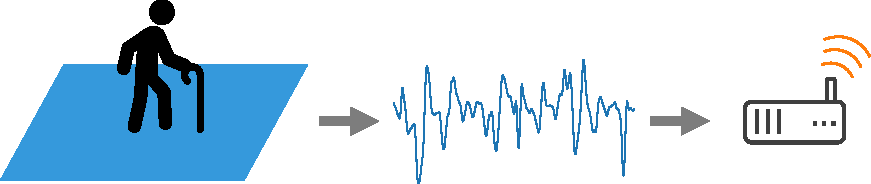
\includegraphics[width=0.95\linewidth]{schema_fall_detector.pdf}\\
    \pause
\end{minipage}\hfill
\begin{minipage}[t]{0.47\linewidth}
        \vspace{0pt}
        \centering\textbf{Tarkett's objective}\\
        \smallskip
        {\textcolor{myblue}{Providing tools for elderly monitoring\\ in nursing homes}}
    
%         \pause
        \medskip
        \centering\textbf{Challenges}
        \begin{itemize}
            \item Signal interpretability (external perturbations, artefacts, unidimensional for one area)
    %         \begin{itemize}
    %             \item Proliferation of sensor-based systems
    %             \item Redundancy, interpretability, external pertubations
    %         \end{itemize}
            \item Real world application (data scarcity, model for embedded systems)
    %         \begin{itemize}
    %             \item Real-time processing in a limited system
    %             \item Convenient hypotheses not granted
    %         \end{itemize}
        \end{itemize}
%         \begin{figure}[h]
%                 \centering
%                 \vspace{0.5cm}
%                 \onslide<2->
\includegraphics[width=0.4\linewidth]{Tarkett-logo_red.jpg}\\[5pt]
%                 \pause
        %         \onslide<2->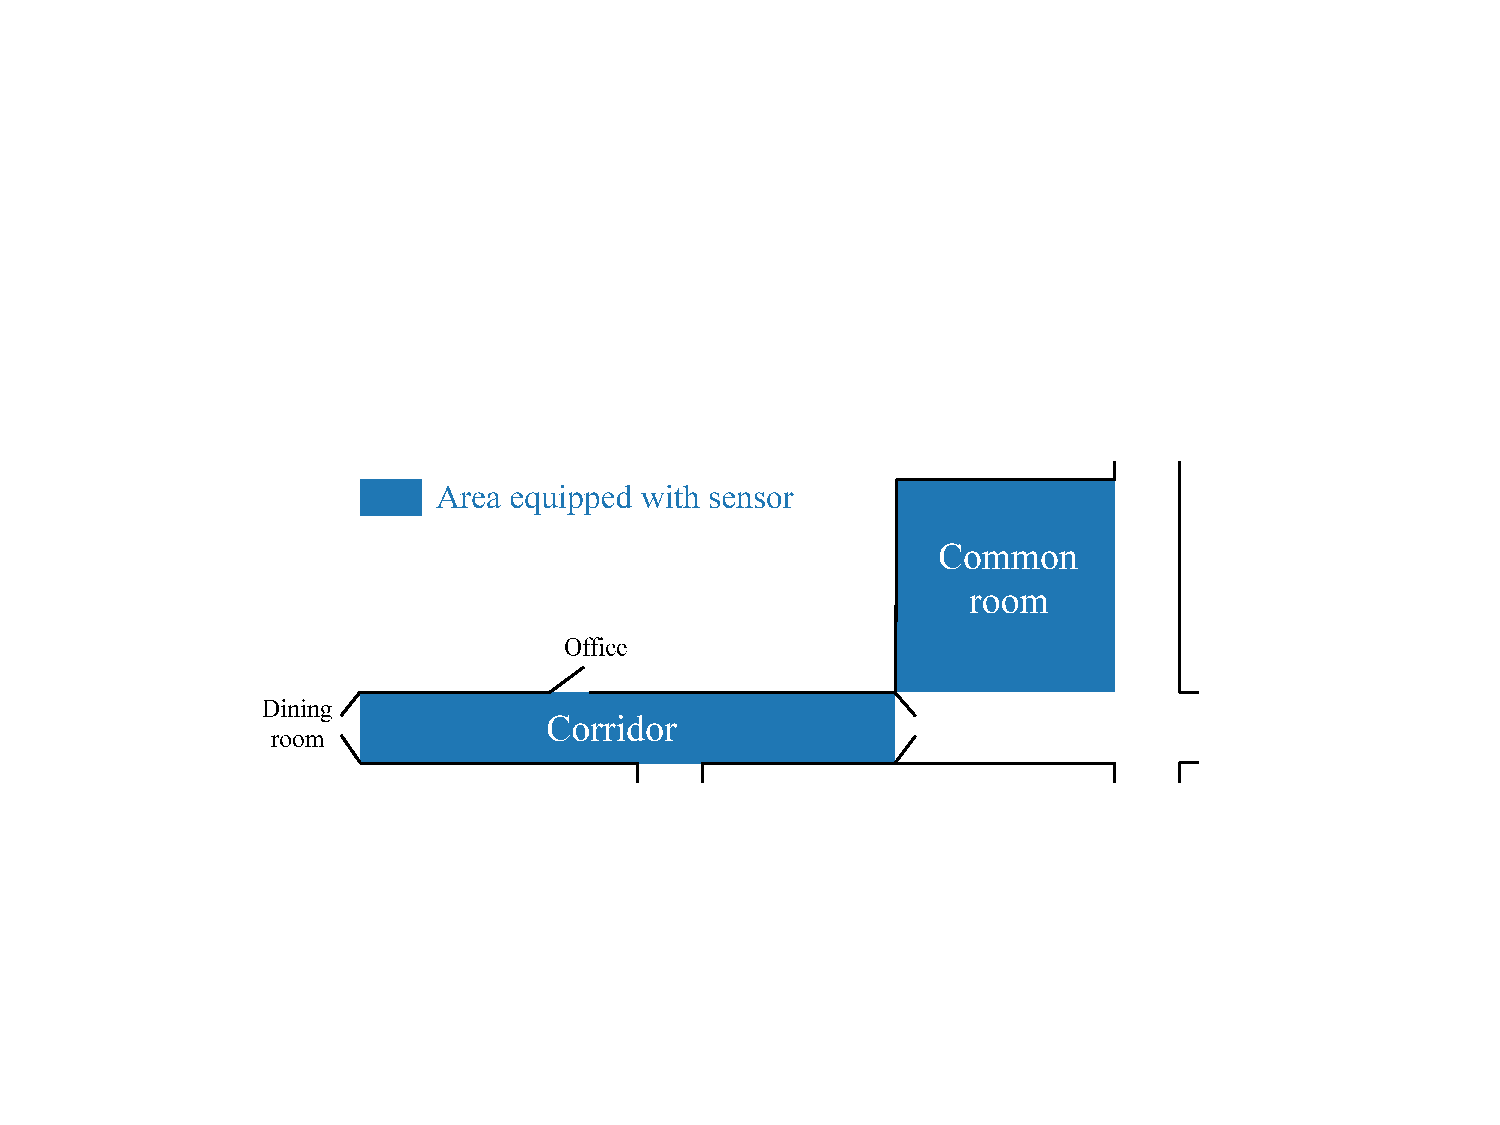
\includegraphics[width=0.6\linewidth, trim= 50 150 50 210, clip]{schema_couloir_plan_blue.pdf}
        %     \end{minipage}
        %     \caption{System installation in a nursing home.}
        %     \label{fig:schema_installation}
%         \end{figure}
%     \bigskip
        \centering
        \begin{minipage}[t]{0.9\linewidth}
            \vspace{0.5pt}
            \centering
            \onslide<2->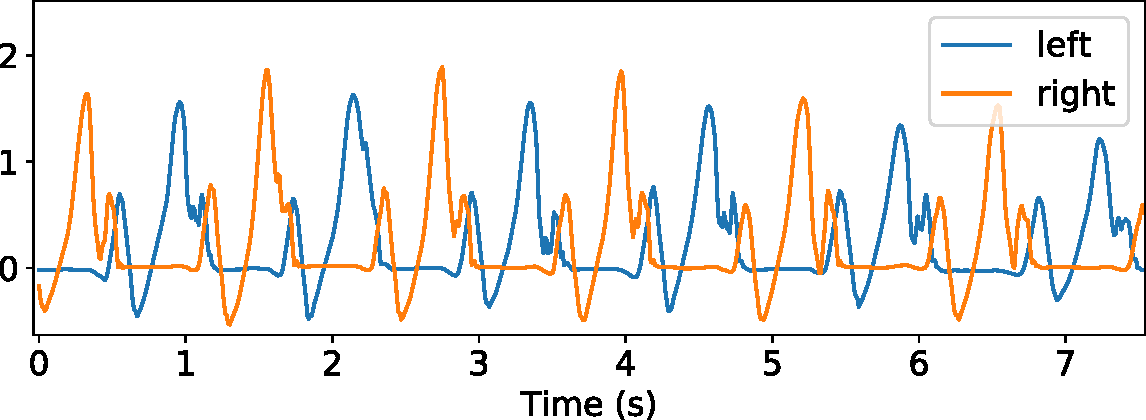
\includegraphics[width=0.7\linewidth]{signal_marche_accelerometre_left_right_epure.pdf}\\
            {\small Walk recorded with accelerometers}
        \end{minipage}\\
        \smallskip
        \begin{minipage}[t]{0.9\linewidth}
            \vspace{0pt}
            \centering
            \onslide<2->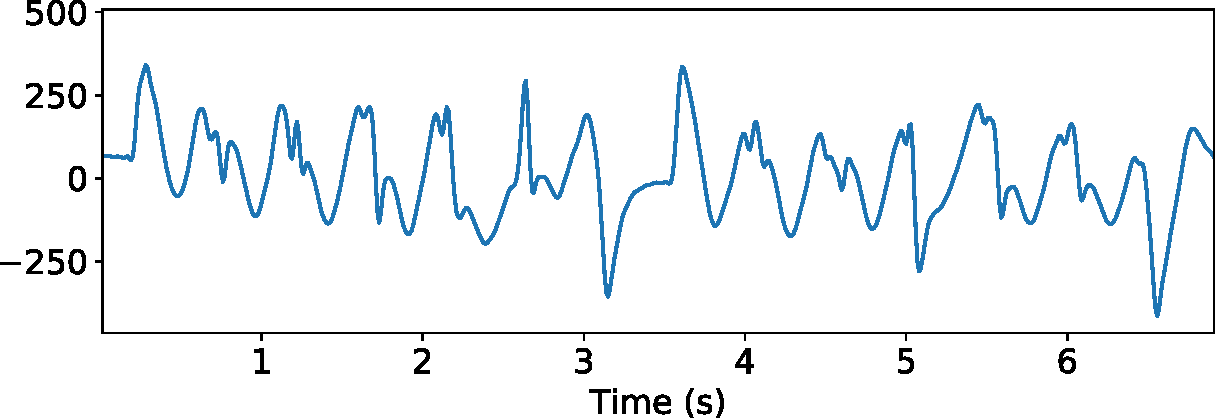
\includegraphics[width=0.75\linewidth]{signal_marche_tarkett_epure.pdf}\\
            {\small Walk recorded with Tarkett's floor sensor}
        \end{minipage}
        
%     \pause
%     \medskip
%     \centering\textbf{Questions}
%     \begin{itemize}
%         \item Is a floor-based system a good idea ?
%         \item How to build a fall detector out of it ?
%         \item How to use real data to improve our model ?
%         \item The signal is unidimensional: can we still distinguish people ?
%     \end{itemize}
\end{minipage}
\end{frame}

\endgroup

% Outline
\begingroup
\setbeamertemplate{headline}{}
\setbeamertemplate{navigation symbols}{}  % remove page number within the group
\setcounter{tocdepth}{1}
\begin{frame}[noframenumbering]{Outline}
% \begin{minipage}[t]{0.49\linewidth}
% \parbox[t]{.85\textwidth}{
%     \begin{minipage}[c][0.65\textheight]{\textwidth}
    \centering
%     \vspace{1.0cm}
    \Large
    \renewcommand{\ratio}{0.5}
%     \tableofcontents
    \vspace{\ratio cm}
    
    \textcolor{myblue}{1. Monitoring systems for fall detection}
    
    \vspace{\ratio cm}
            
     \textcolor{myblue}{       2. Fall detection using a floor sensor and machine learning}
            
    \vspace{\ratio cm}
    
     \textcolor{myblue}{      3. Transfer learning from experimental setup to operational data}
     
    \vspace{\ratio cm}
            
     \textcolor{myblue}{       4. Elderly activity recognition with convolutional neural networks}
     
    \vspace{\ratio cm}
    
     \textcolor{myblue}{       5. Conclusion}
%     \end{minipage}
% }
% \end{minipage}
\end{frame}
\endgroup

\section{Monitoring systems}

\begingroup
\setbeamertemplate{navigation symbols}{}  % remove page number within the group
\begin{frame}[noframenumbering]{}
    \centering
    \vspace{3cm}
    \Huge
    \textcolor{myblue}{Monitoring systems for fall detection}
\end{frame}
\endgroup


\subsection{Sensors}

\begin{frame}{Sensors}{}
    
    \begin{minipage}[t]{0.49\linewidth}
        \vspace{0pt}
What makes a good monitoring system ?
        \begin{itemize}
            \item coverage and occlusion
            \item intrusiveness
            \item signal quality / information
            \item robustness
            \item ease of installation / use
            \item scalability
        \end{itemize}

    \end{minipage}\hfill
    \begin{minipage}[t]{0.49\linewidth}
        \vspace{0pt}
        \begin{overprint}
%             \onslide<2>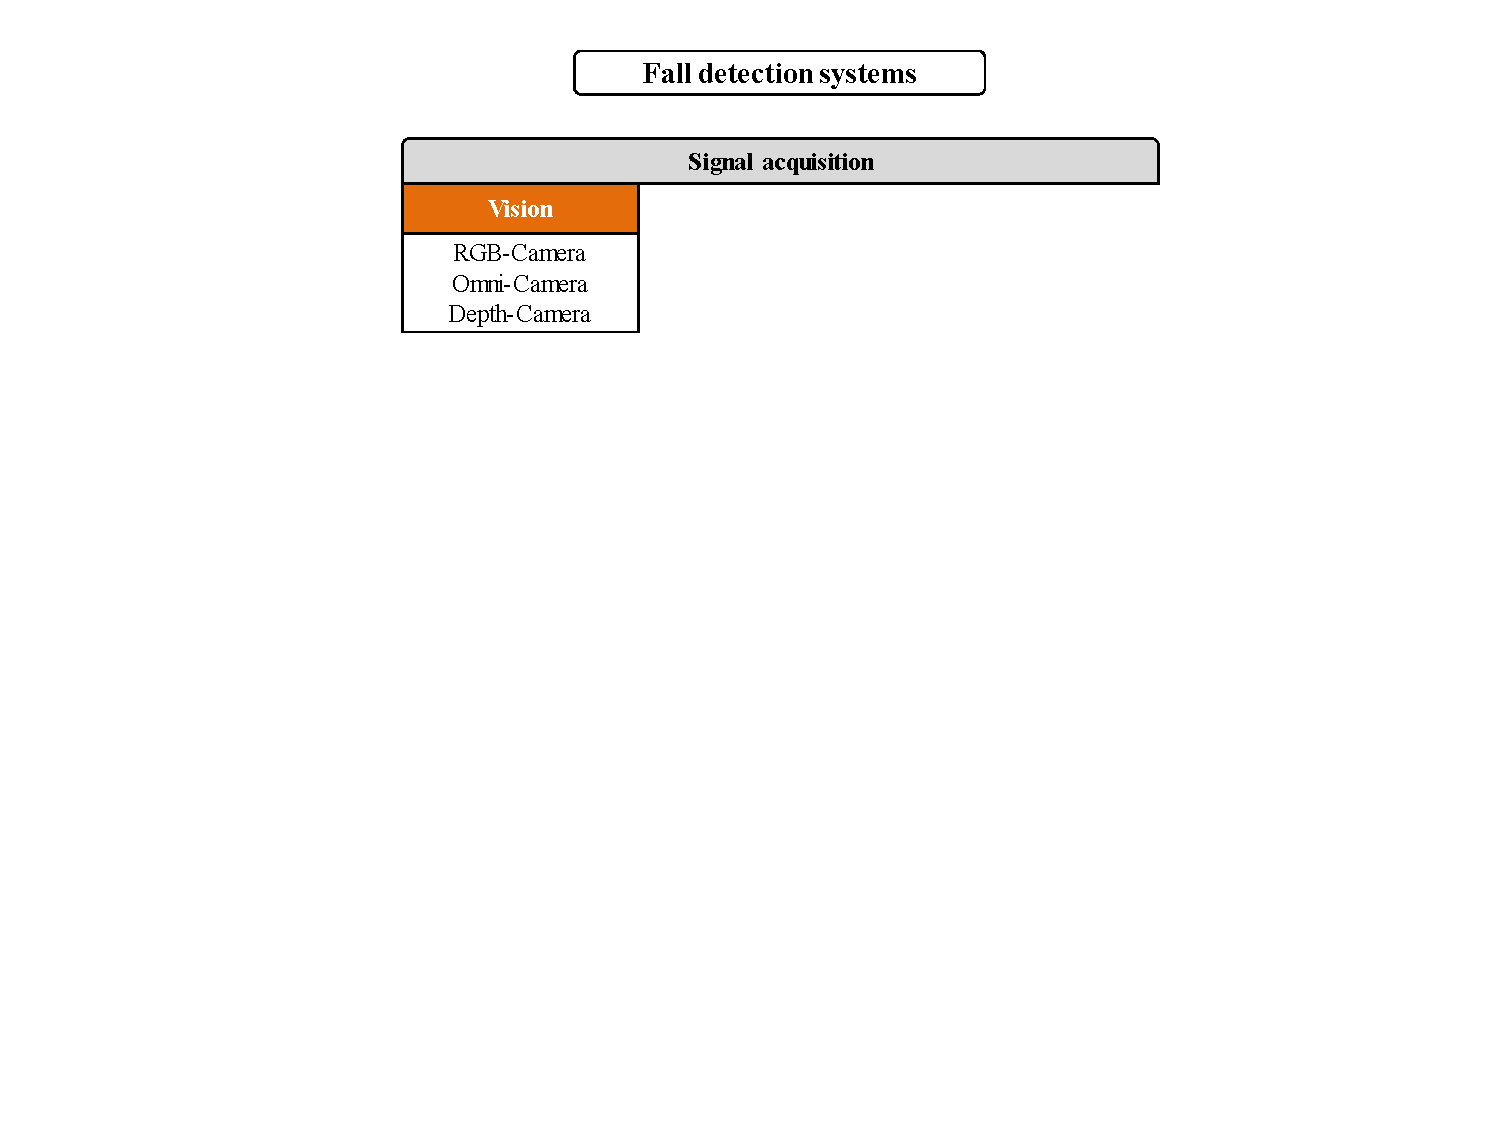
\includegraphics[width=\linewidth, trim={190 250 150 60}, clip]{fall_systems_1_1-14.pdf}
%             \onslide<3>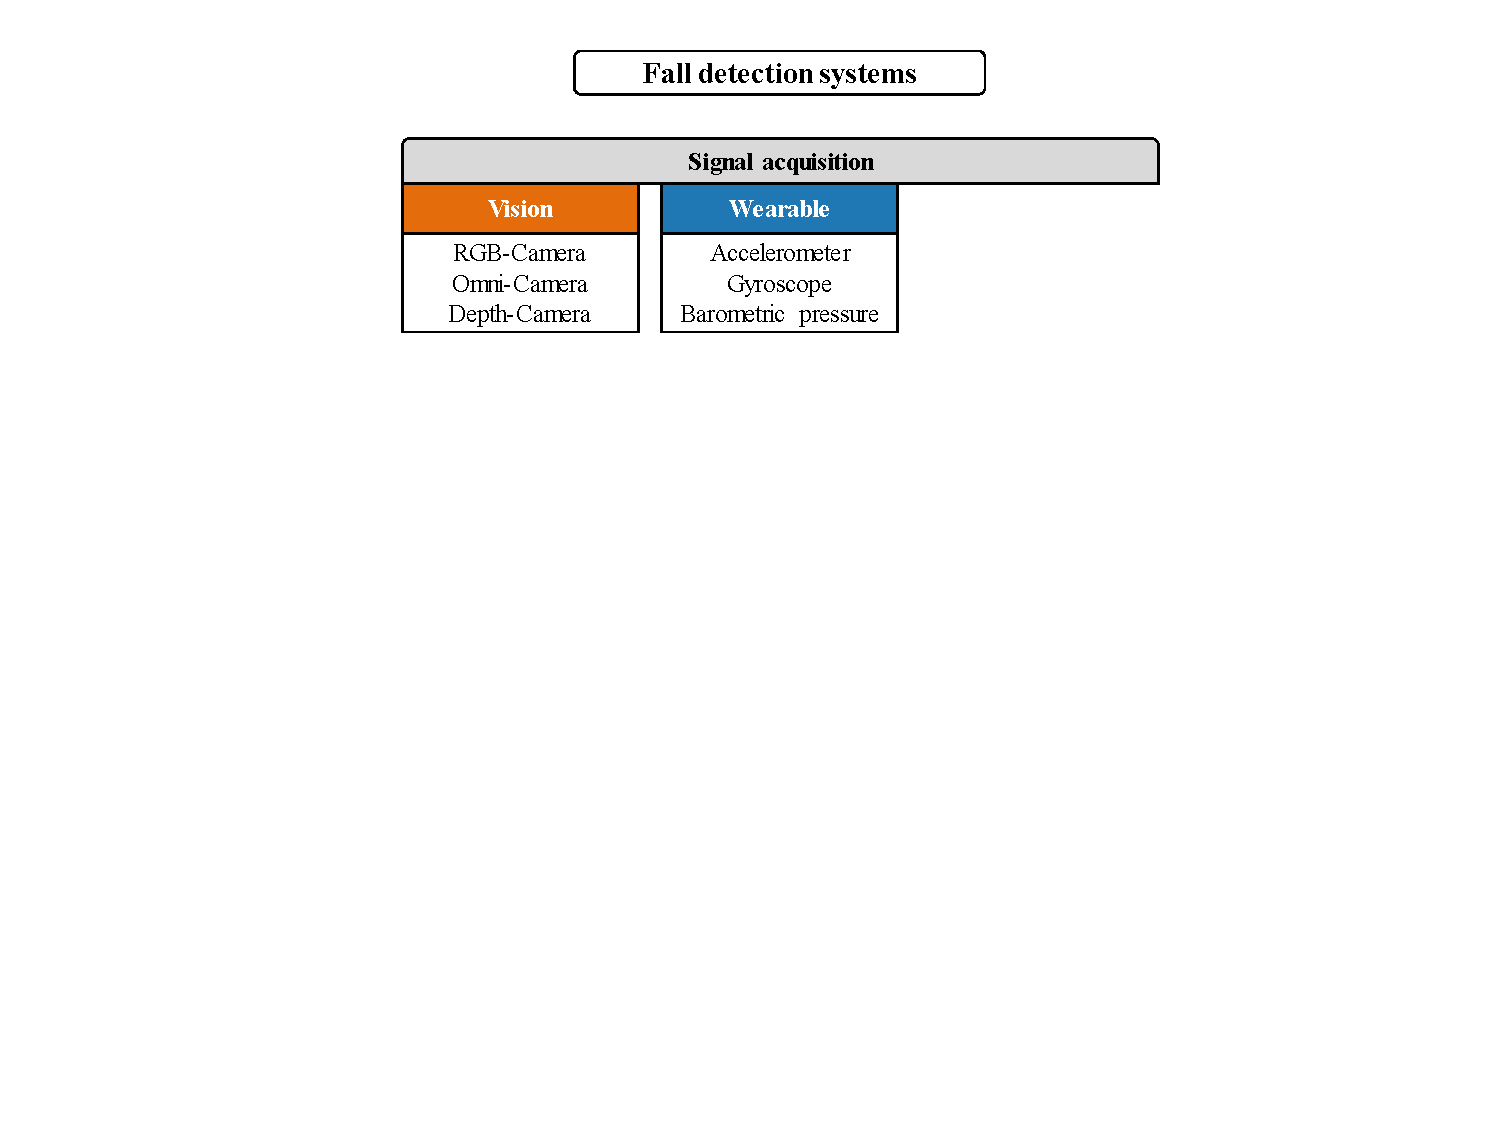
\includegraphics[width=\linewidth, trim={190 250 150 60}, clip]{fall_systems_1_2-14.pdf}
%             \onslide<4>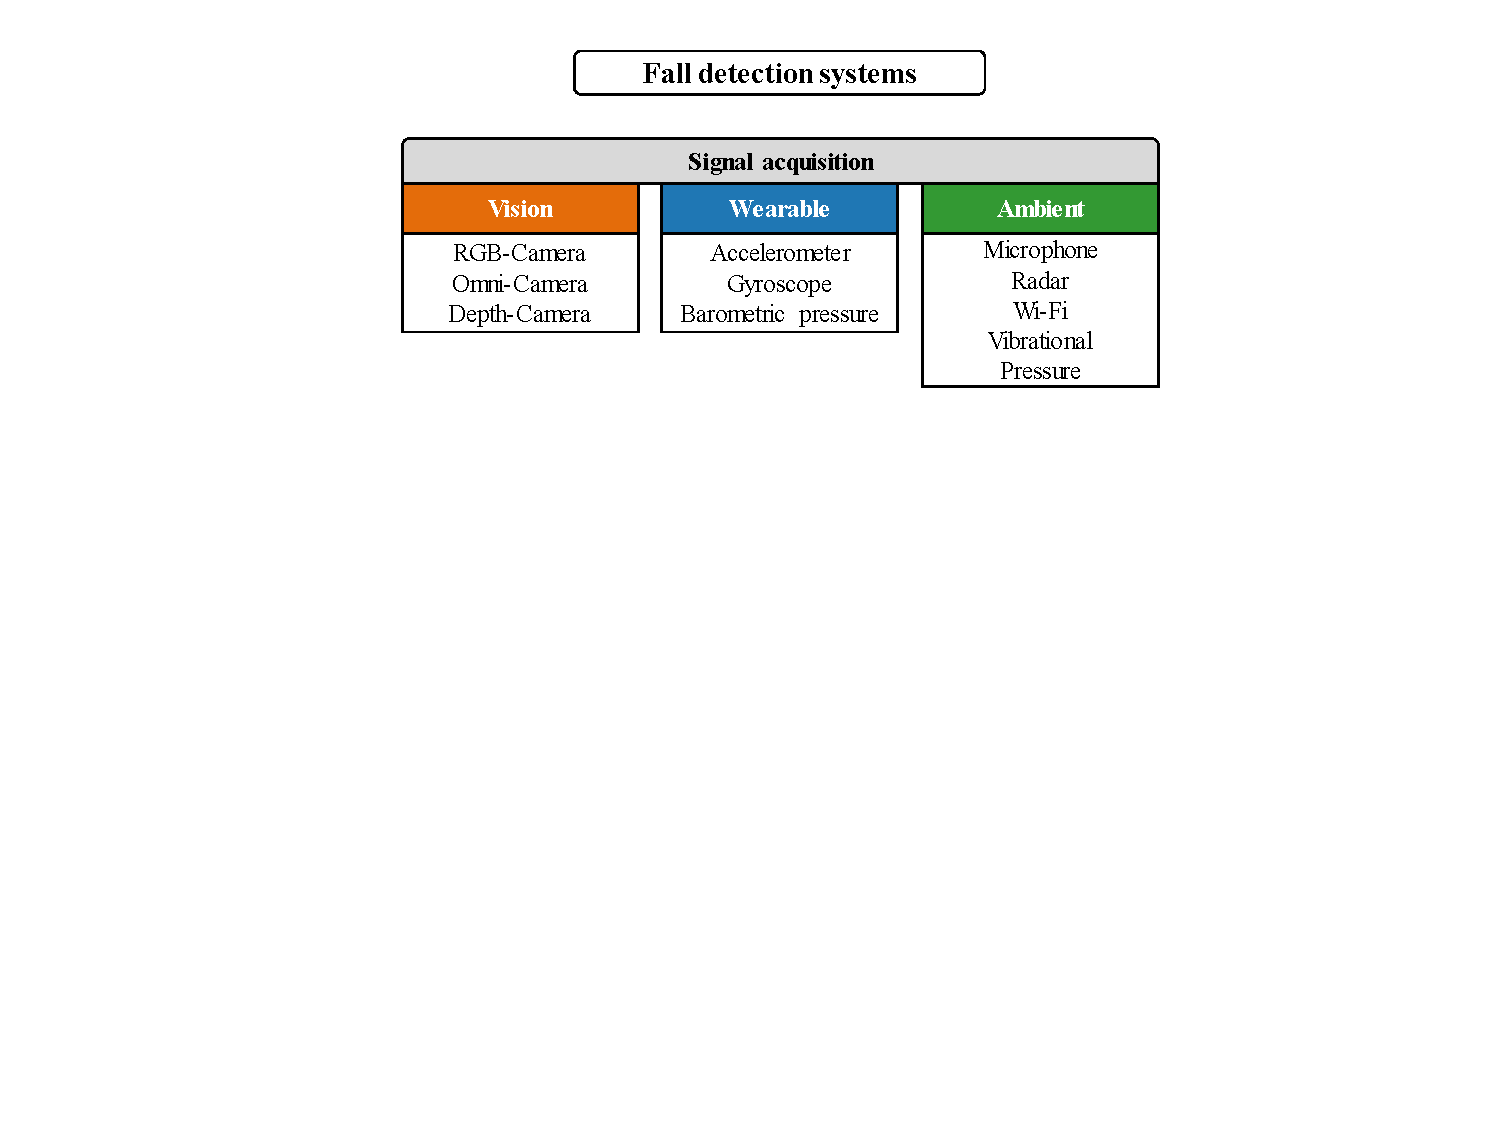
\includegraphics[width=\linewidth, trim={190 250 150 60}, clip]{fall_systems_1_3-14.pdf}
            \onslide<2>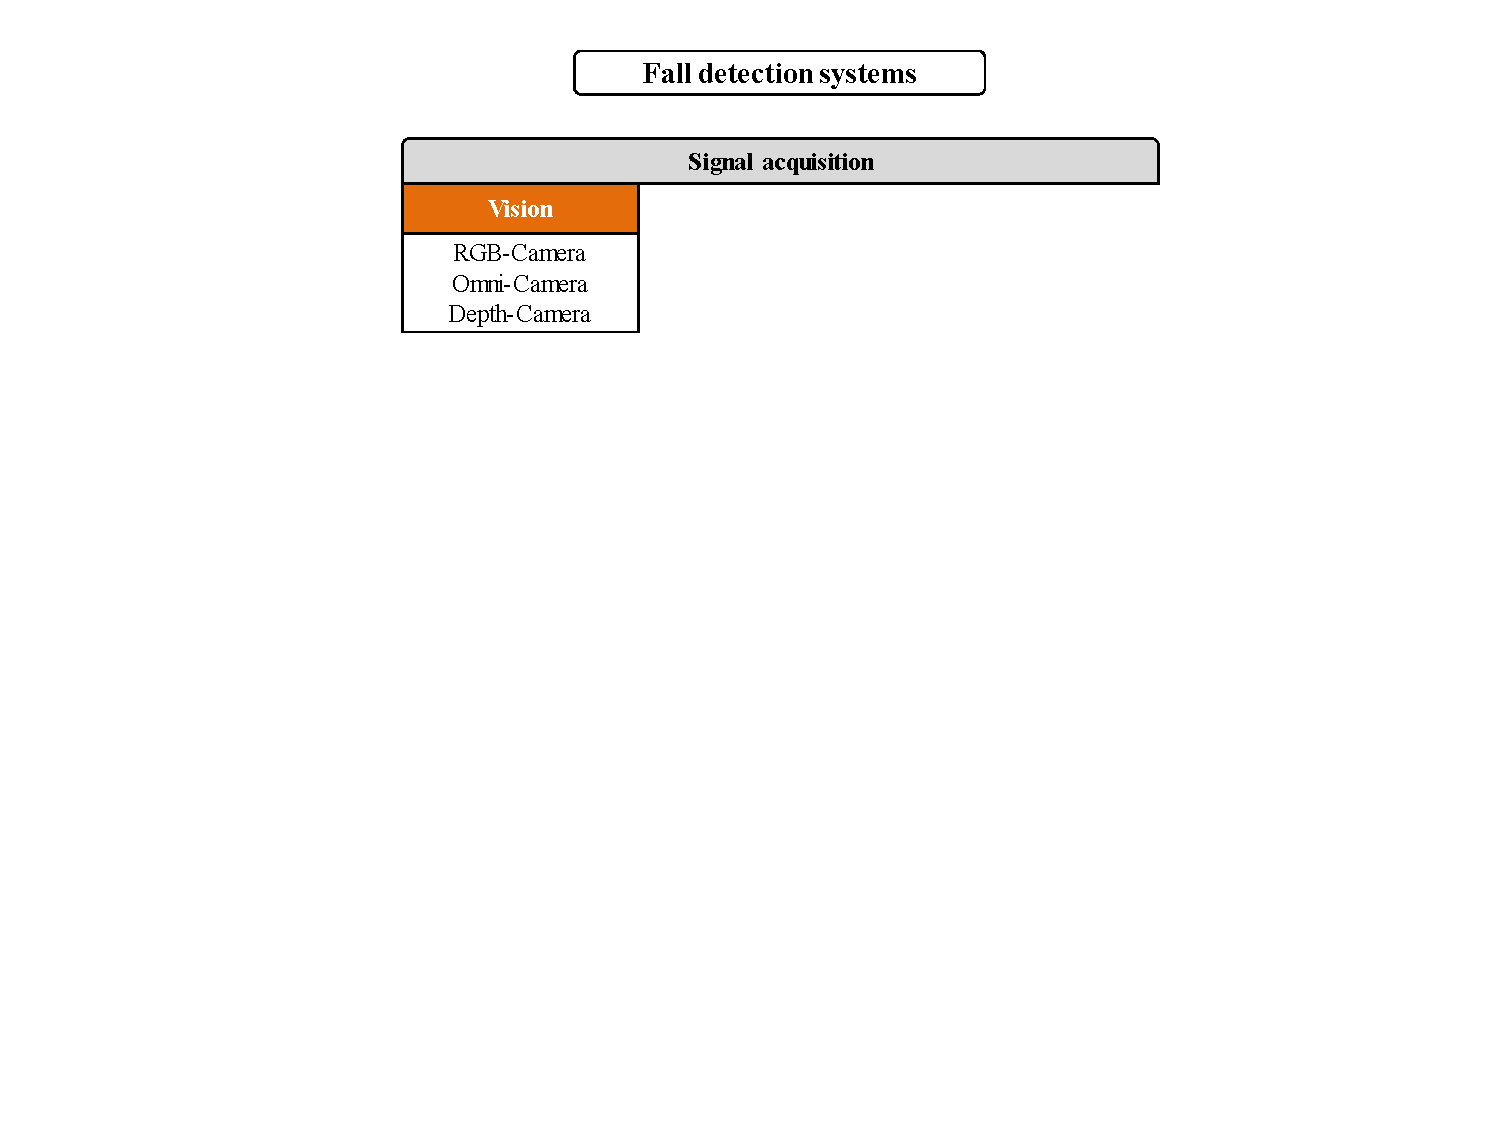
\includegraphics[width=\linewidth, trim={190 250 150 60}, clip]{schemas_fallsystems_1_14.pdf}
            \onslide<3>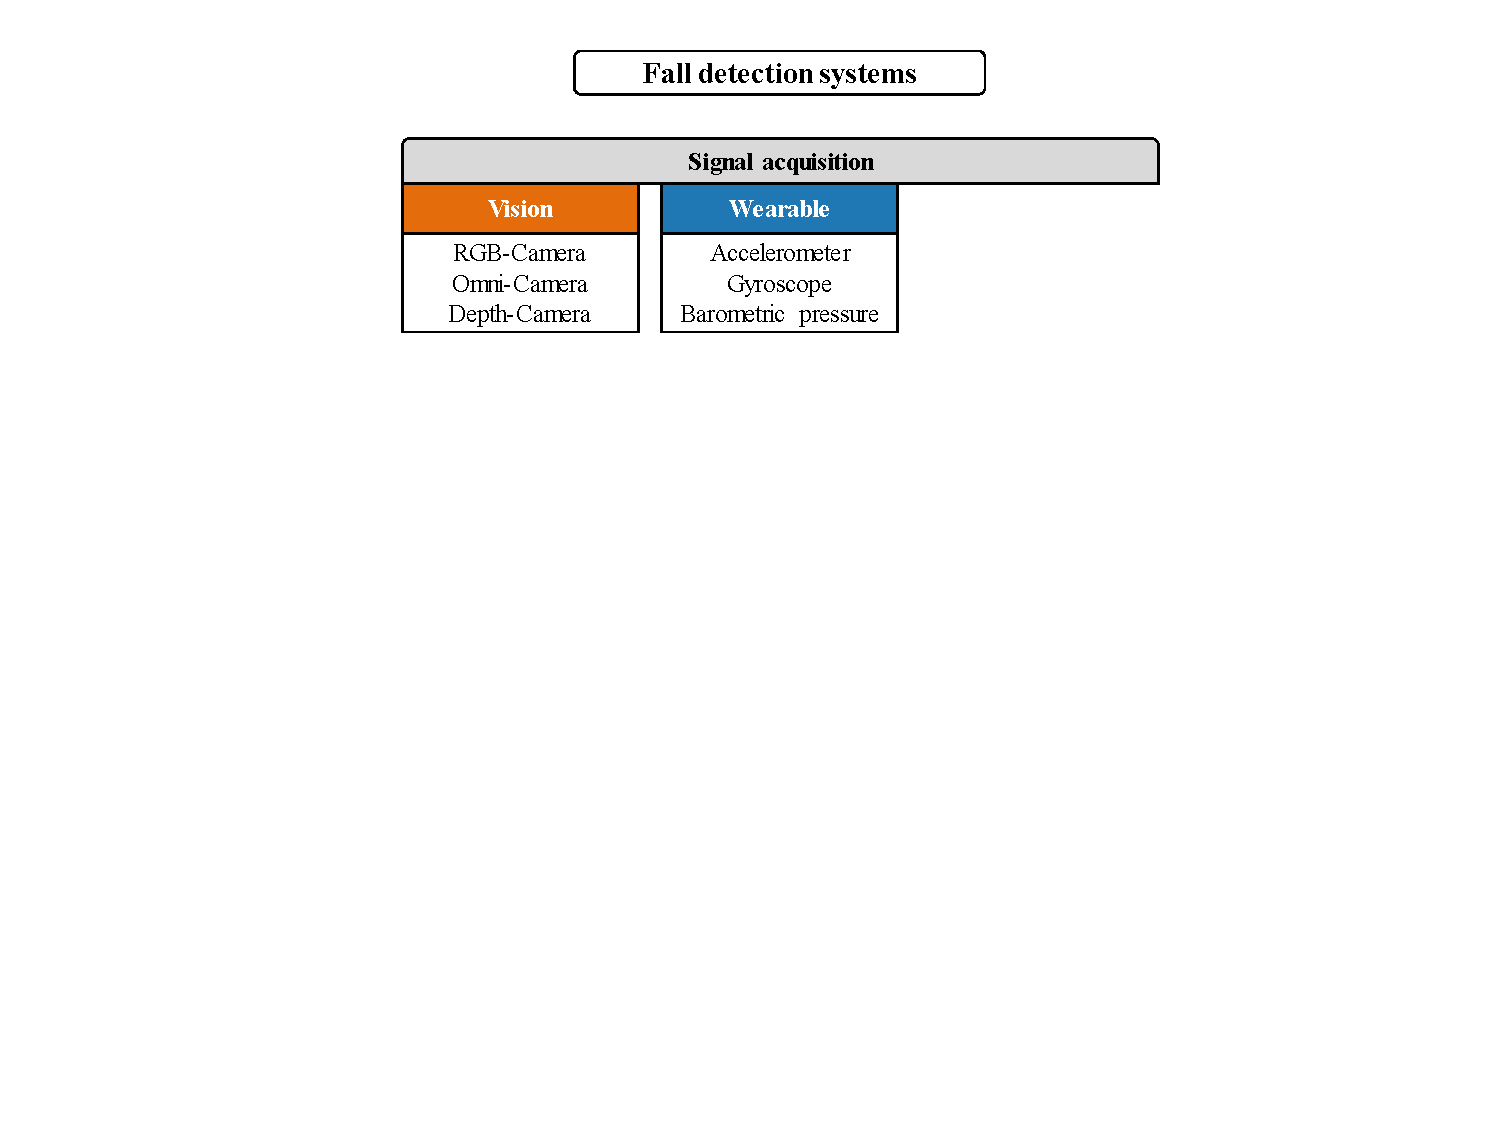
\includegraphics[width=\linewidth, trim={190 250 150 60}, clip]{schemas_fallsystems_2_14.pdf}
            \onslide<4>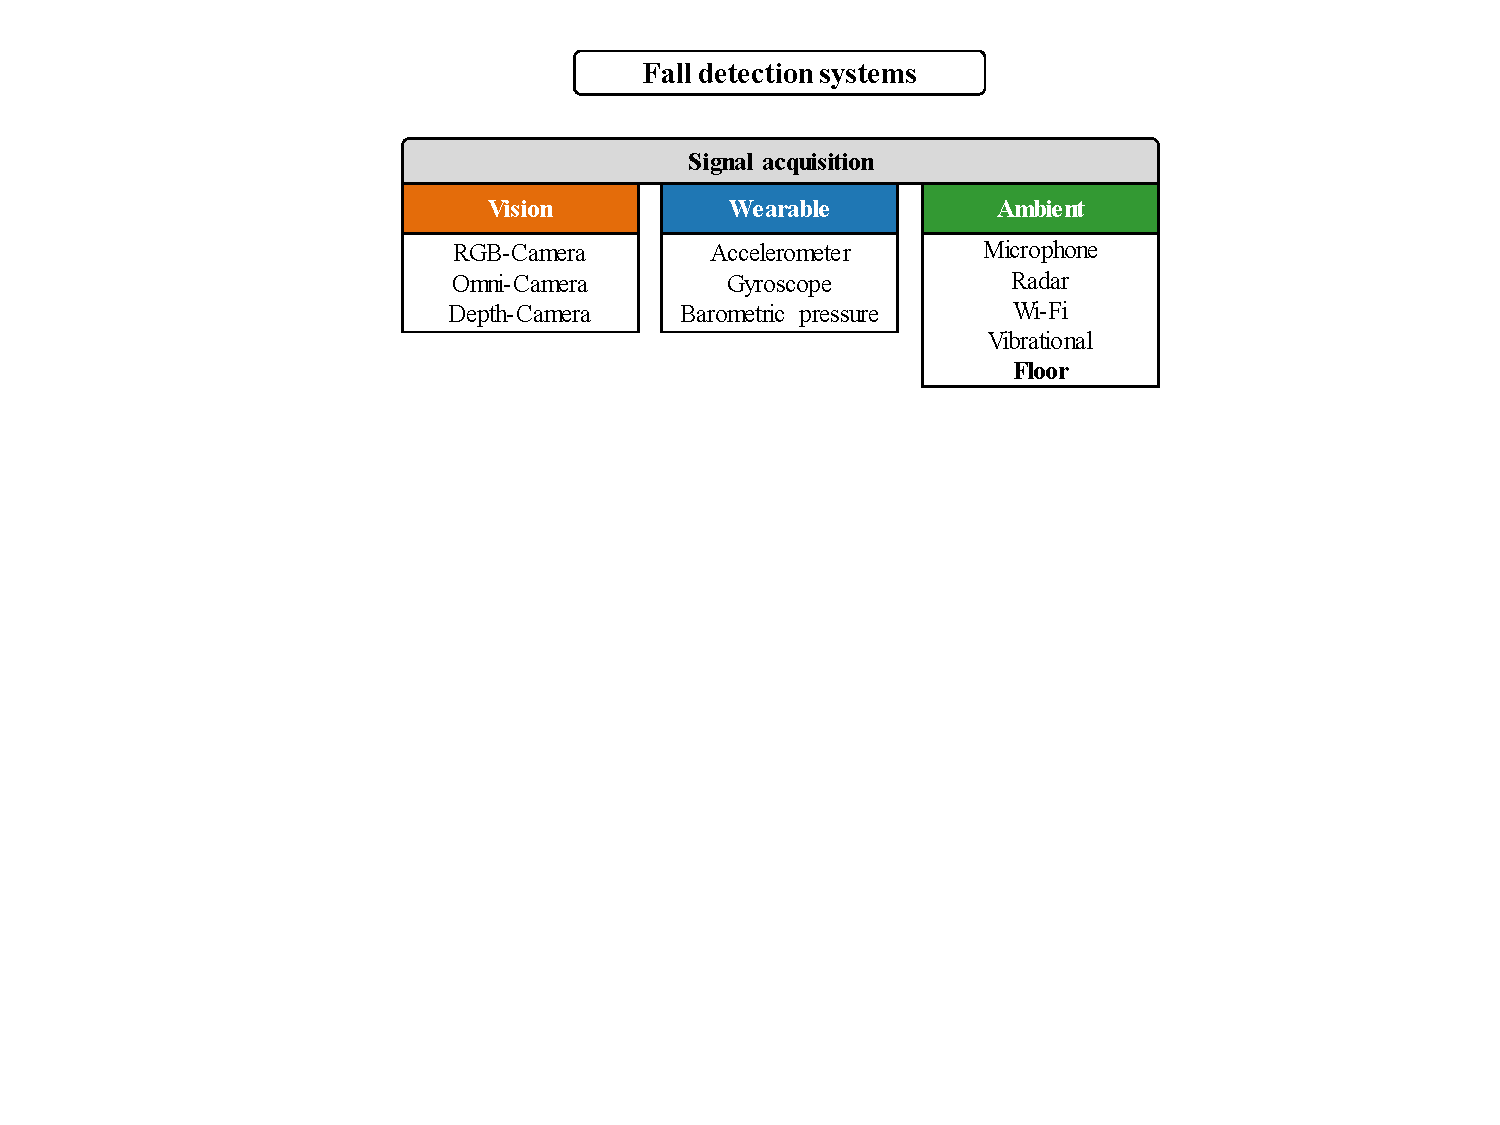
\includegraphics[width=\linewidth, trim={190 250 150 60}, clip]{schemas_fallsystems_3_14.pdf}
        \end{overprint}
    \end{minipage}
% \end{minipage}

\vspace{-0.8cm}
% \onslide<1>{
\renewcommand{\arraystretch}{1.1}
\newcommand{\myvar}{45}
\begin{table}[]
\centering
\footnotesize
% \small
    \begin{tabular}{l c c c c c c c}
%     \hline
    Criteria & \onslide<2->{\rotatebox{\myvar}{RGB cam} & \rotatebox{\myvar}{Depth cam}} & \onslide<3->{\rotatebox{\myvar}{Wearable}} & \onslide<4->{\rotatebox{\myvar}{Acoustic} & \rotatebox{\myvar}{Radar / Wi-Fi} & \rotatebox{\myvar}{Vibration} & \rotatebox{\myvar}{\textbf{Floor}}} \\
    \midrule
    Coverage/Occlusion & \onslide<2->{\starb\starw\starw & \starb\starw\starw} & \onslide<3->{\starb\starb\starb} & \onslide<4->{\starb\starb\starw & \starb\starw\starw & \starb\starb\starb & \starb\starb\starb} \\
    Intrusiveness & \onslide<2->{\starb\starw\starw & \starb\starw\starw} & \onslide<3->{\starb\starb\starw} & \onslide<4->{\starb\starw\starw & \starb\starb\starw & \starb\starb\starb & \starb\starb\starb} \\
    Signal quality / info &\onslide<2->{\starb\starb\starb & \starb\starb\starb} & \onslide<3->{\starb\starb\starw} & \onslide<4->{\starb\starb\starw & \starb\starw\starw & \starb\starb\starw & \starb\starb\starw} \\
    Robustness & \onslide<2->{\starb\starb\starw & \starb\starb\starb} & \onslide<3->{\starb\starb\starb} & \onslide<4->{\starb\starw\starw & \starb\starw\starw & \starb\starw\starw & \starb\starb\starw} \\
    Ease of instal. / use & \onslide<2->{\starb\starw\starw & \starb\starw\starw} & \onslide<3->{\starb\starb\starw} & \onslide<4->{\starb\starb\starw & \starb\starb\starw & \starb\starb\starb & \starb\starw\starw} \\
    Scalability & \onslide<2->{\starb\starw\starw & \starb\starw\starw} & \onslide<3->{\starb\starb\starb} & \onslide<4->{\starb\starb\starw & \starb\starw\starw & \starb\starb\starw & \starb\starb\starb} \\
    \midrule
    \end{tabular}
% \caption{Sensors evaluation over key criteria for patient monitoring systems.}
\label{tab:fall_detection_sensors_comparison}
\end{table}
\renewcommand{\arraystretch}{1.0}
% }

\end{frame}

\subsection{Information extraction}
\begin{frame}{Information extraction}

% \begin{minipage}[t]{\linewidth}
    \begin{minipage}[t]{0.49\linewidth}
    \vspace{0pt}
    How to process the inputs ?
    \begin{itemize}
        \item All systems use feature extraction
        \item The ``level'' of feature engineering depends on the complexity / dimensionality of the input signal
    \end{itemize}
    \onslide<1>{
    \vspace{0.2cm}
    How to deal with feature signals ?
    \begin{itemize}
        \item Use simple thresholds
        \item Use them as feature vectors for classification models (anomaly detection, classical supervised models)
    \end{itemize}
    }
%     \begin{tcolorbox}[title=Time series classification]
%         \begin{enumerate}
%             \item Series as \emph{sequences}
%             \begin{itemize}
%                 \item Distance-based methods
%             \end{itemize}
%             \item Series as \emph{feature vectors}
%             \begin{itemize}
%                 \item Computing several measures over a fixed size
%                 \item Classification models
%                 (Anomaly detection, classical supervised models...)
%             \end{itemize}
%         \end{enumerate}
%     \end{tcolorbox}
%     \vfill
%     \vspace{10cm}
    \end{minipage}
    \hfill
    \begin{minipage}[t]{0.49\linewidth}
    \vspace{0pt}
        \begin{overprint}
%             \onslide<1>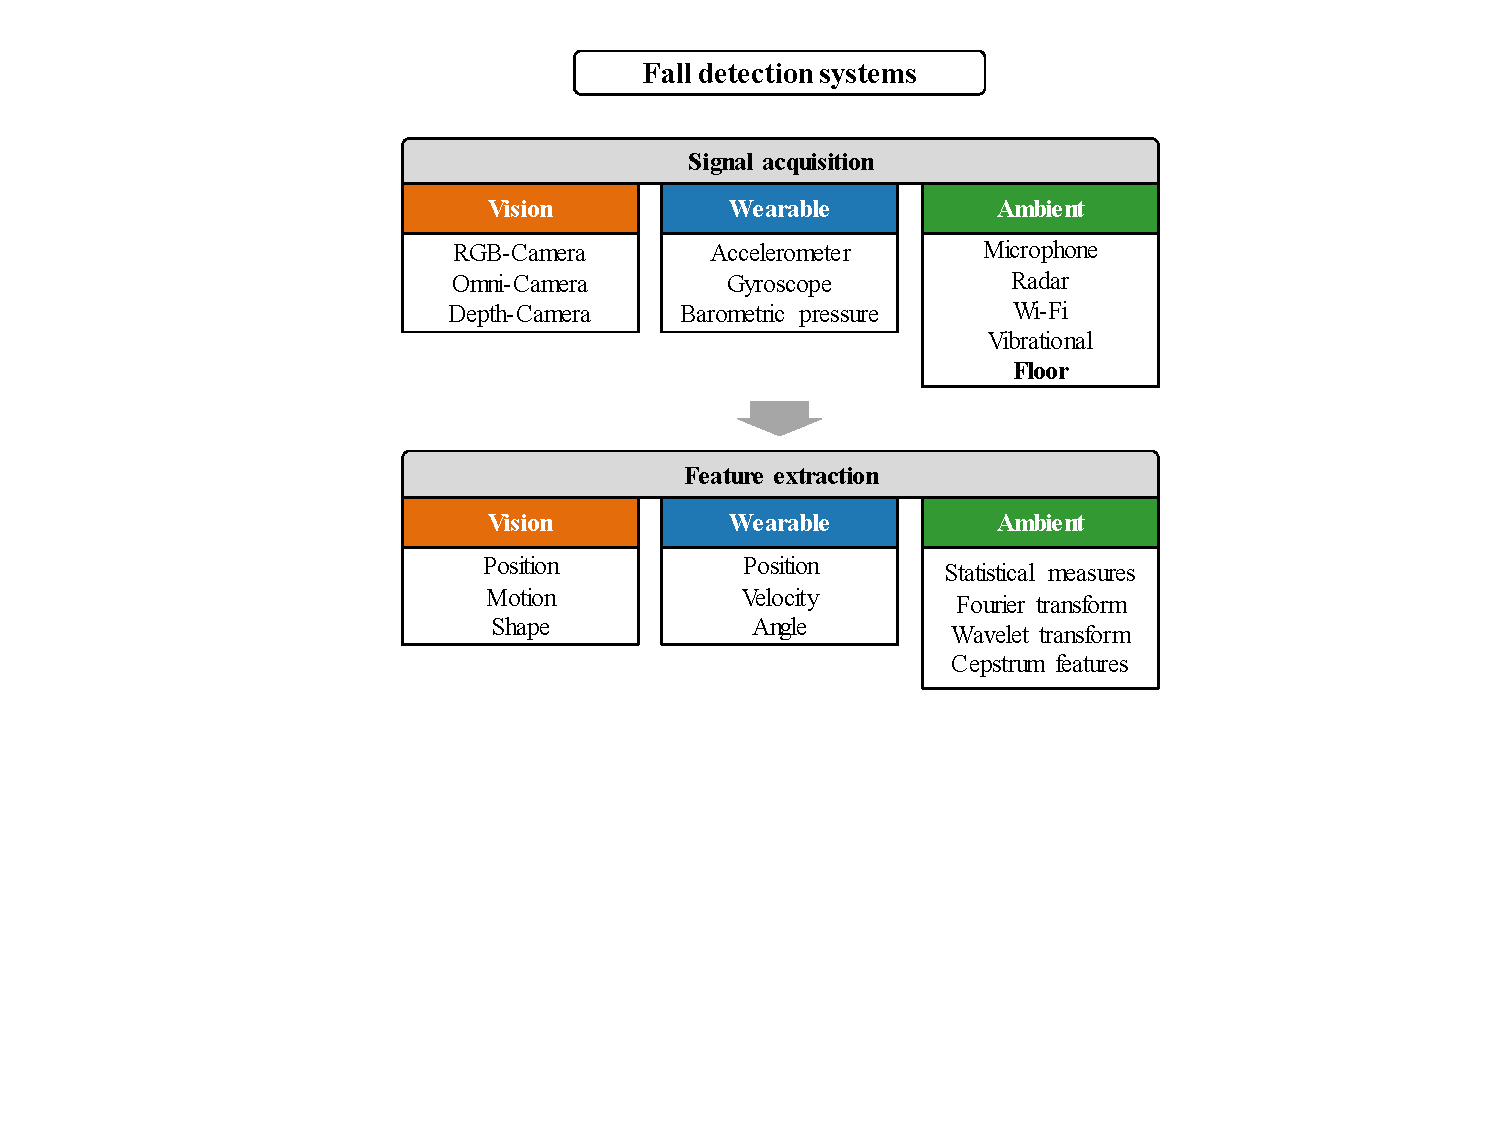
\includegraphics[width=\linewidth, trim={190 50 150 60}, clip]{schemas_fallsystems_4_14.pdf}
            \onslide<1>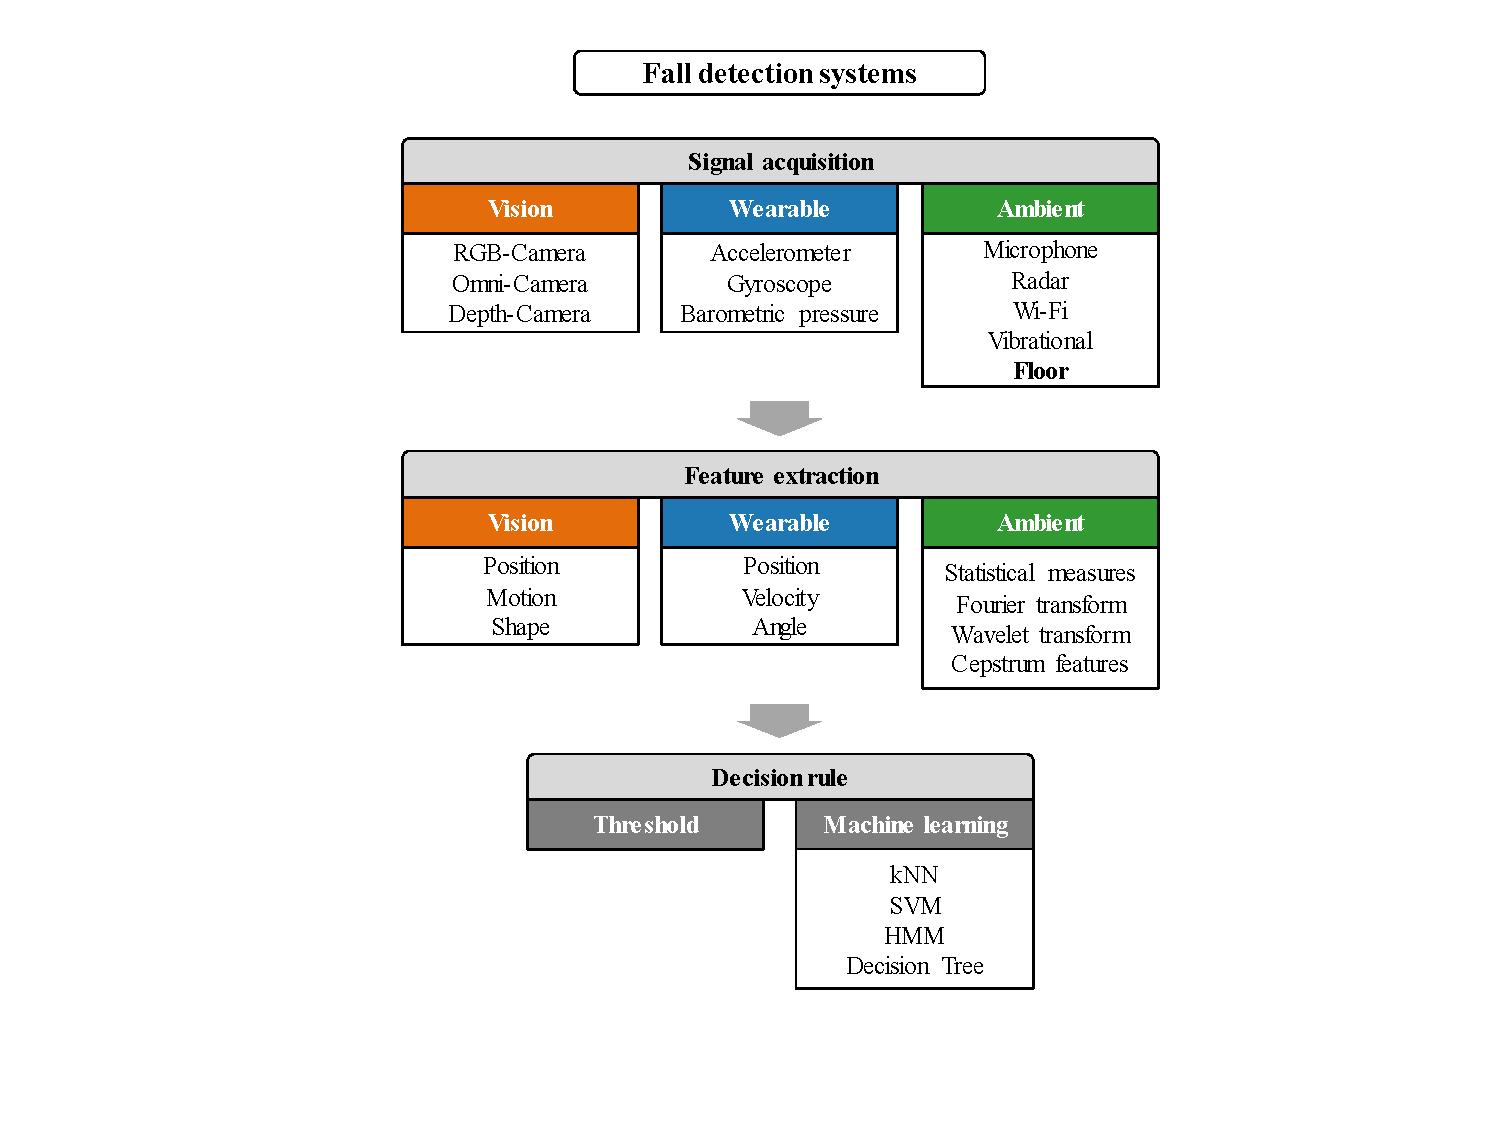
\includegraphics[width=\linewidth, trim={190 50 150 60}, clip]{schemas_fallsystems_5_14.pdf}
        \end{overprint}
    \end{minipage}
% \end{minipage}
\end{frame}




\section{Fall detection}

\begingroup
\setbeamertemplate{navigation symbols}{}  % remove page number within the group
\begin{frame}[noframenumbering]{}
    \centering
    \vspace{3cm}
    \Huge
    \textcolor{myblue}{Fall detection using a floor sensor and machine learning}
\end{frame}
\endgroup

\subsection{Tarkett sensor}
\begin{frame}{Tarkett sensor}
% \begin{figure}[ht]
\begin{minipage}[t]{0.35\linewidth}
    \vspace{0pt}
    \begin{itemize}
        \item Piezoelectric principle: $$d = \frac{Q}{F}\;,$$ (simple version) with d the \emph{piezoelectric constant}.\\
        When stressed or squeezed, the material emits charges.\\
        \pause
        \item How does this look like ?\\
            0.3 mm thick and 60 cm wide roll with customizable length
        \pause
        \item How is it installed ?\\
            \begin{itemize}
                \item Under the flooring
                \item Several connected bands for each area, hence one area corresponds to one input
            \end{itemize}

    \end{itemize}
\end{minipage}\hfill
\begin{minipage}[t]{0.64\linewidth}
    \vspace{0pt}
% \begin{minipage}{\linewidth}
    \centering
    % left bottom right top
    \onslide<1->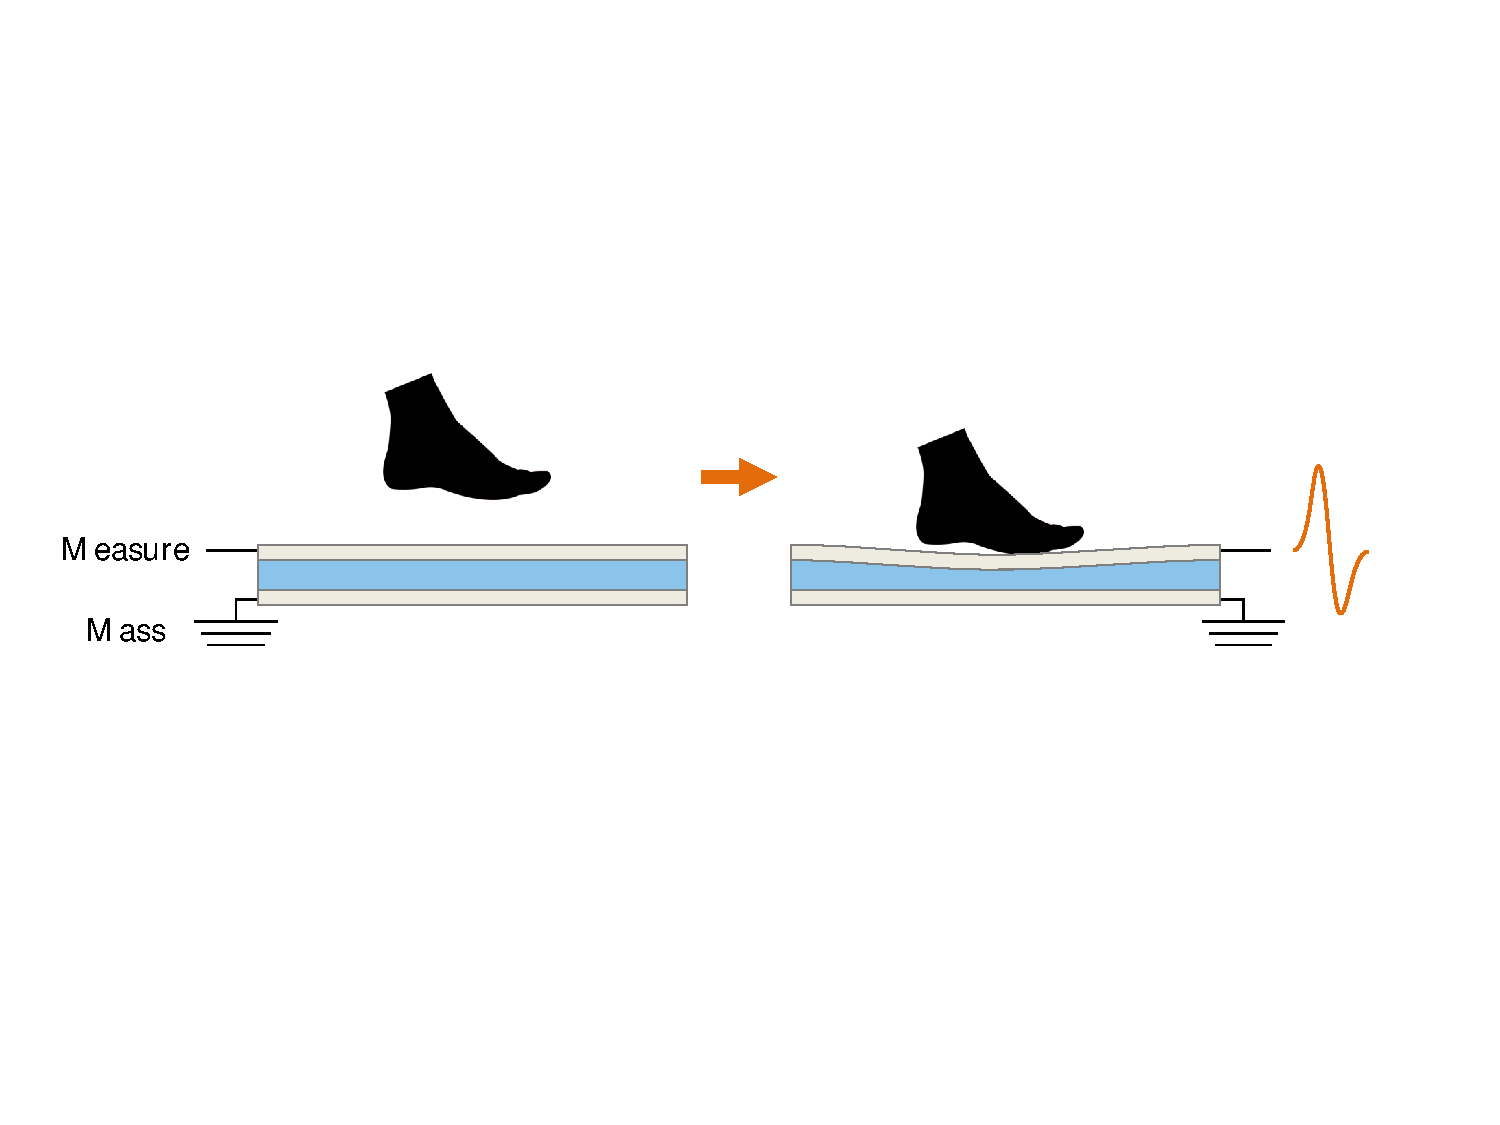
\includegraphics[width=0.9\linewidth, trim={20 220 60 170}, clip]{schema_piezo.pdf}\\
% \caption{Piezoelectric sensor principle.
%          When deformed, the piezoelectric material emits charges, hence a current can be measured in output.
%          }
% \label{fig:schema_piezoelectric}
% \end{figure}
%     \renewcommand{\ratio}{0.4}
    \begin{minipage}[t]{0.49\linewidth}
        \centering
        \onslide<2->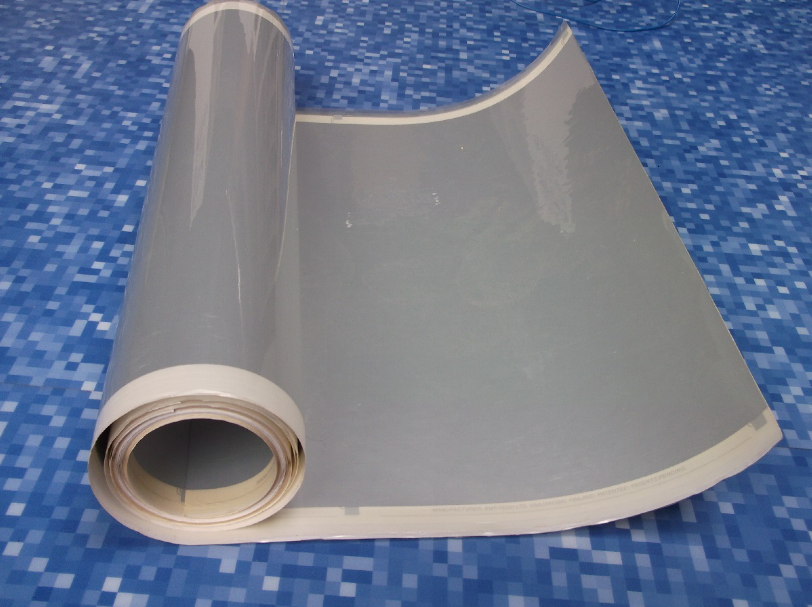
\includegraphics[width=\linewidth, height=1.9cm, keepaspectratio, trim={0 0 0 0}, clip]{photo_capteur_rouleau.png}\\
%         \small Roll of sensor
    \end{minipage}
    \begin{minipage}[t]{0.49\linewidth}
        \centering
        \onslide<2->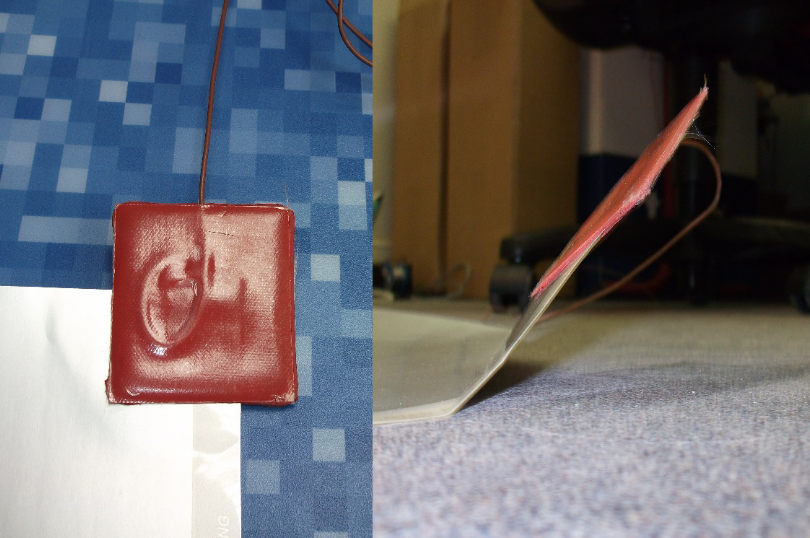
\includegraphics[width=\linewidth, height=1.9cm, keepaspectratio, trim={0 0 0 0}, clip]{photo_capteur_connecteur.png}\\
%         \small Connector
    \end{minipage}
    
% \begin{minipage}[t]{\linewidth}
    \begin{minipage}[b]{0.45\linewidth}
    \centering
    % left bottom right top
    \onslide<3->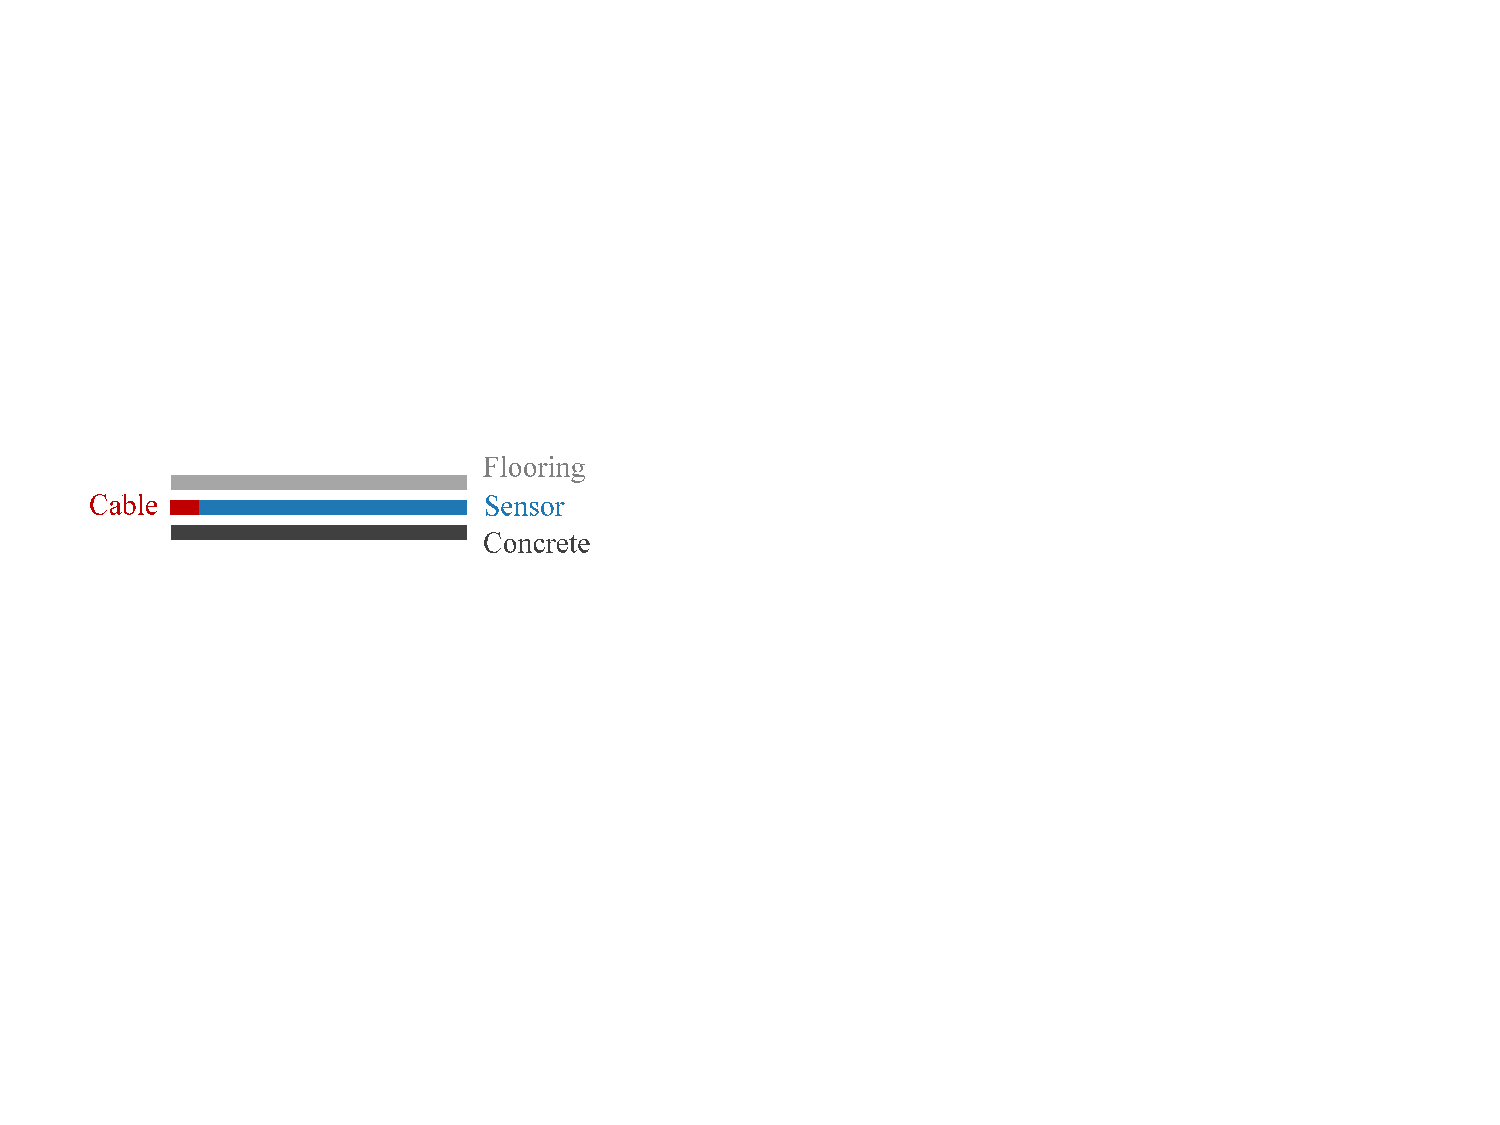
\includegraphics[width=0.95\linewidth, trim={20 260 430 200}, clip]{schema_sensor_installation_3.pdf}
    
%     \small Sensor set up
    \end{minipage}
    \hfill
    \begin{minipage}[b]{0.54\linewidth}
    \centering
    \onslide<3->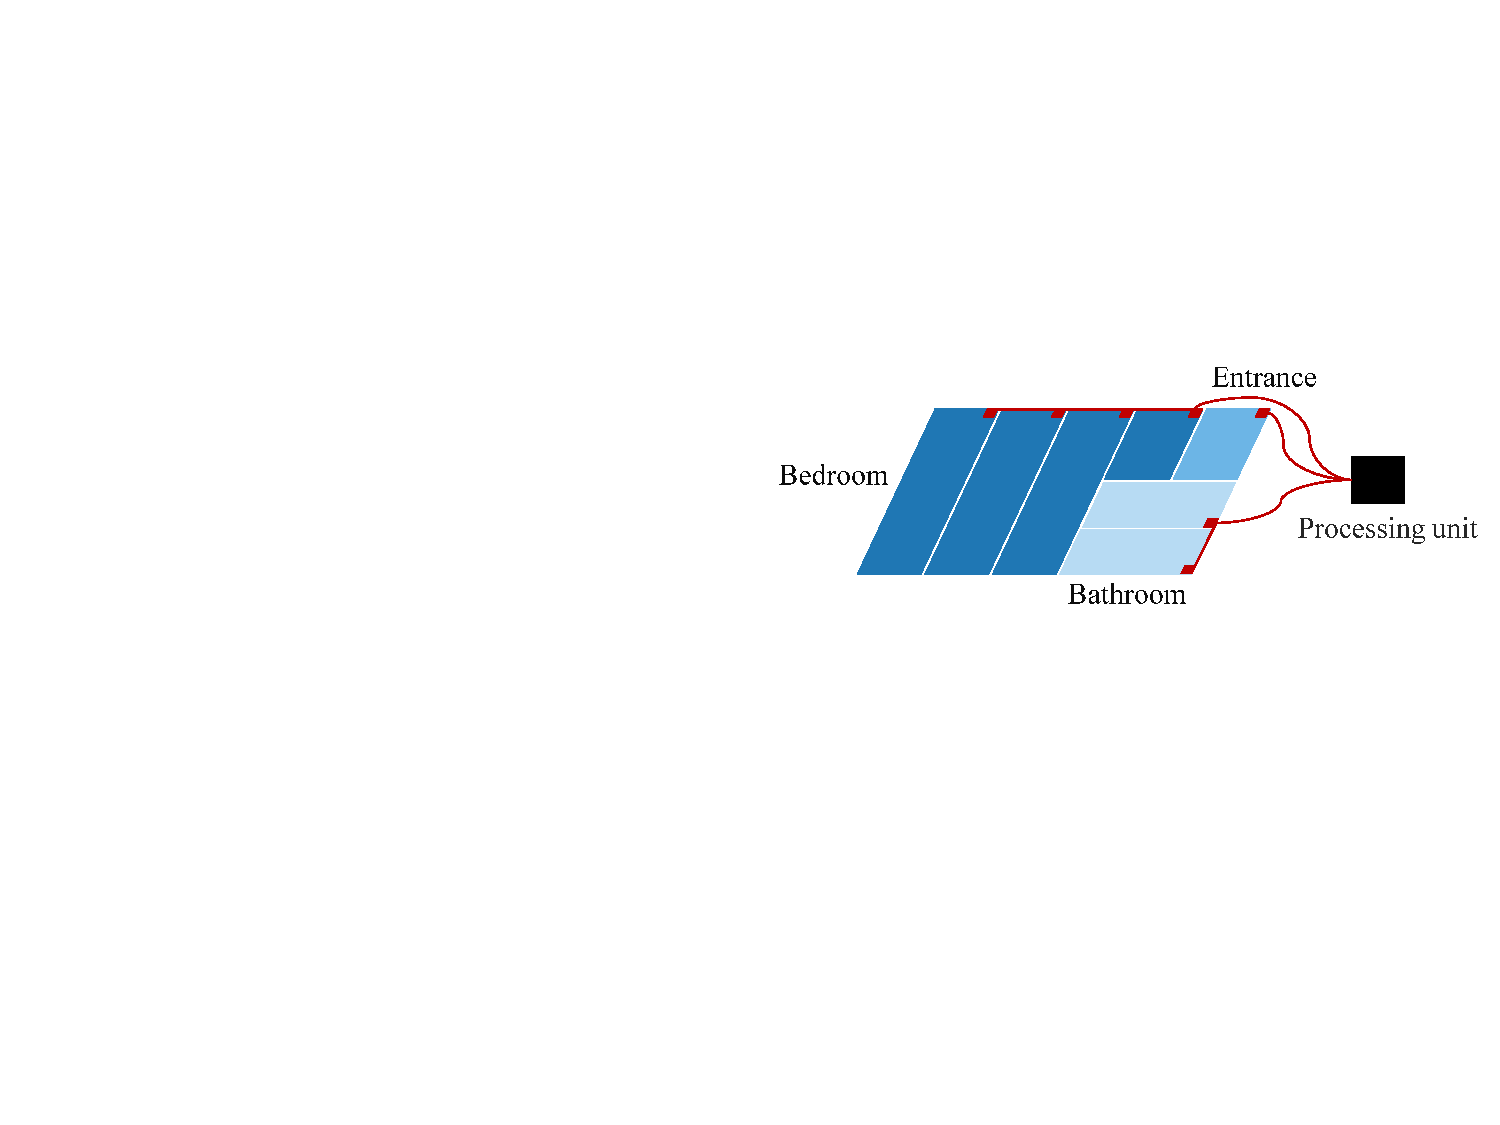
\includegraphics[width=\linewidth, trim={360 240 5 160}, clip]{schema_sensor_installation_room_3.pdf}
    
%     \small Room equipped with the system
    \end{minipage}
% \end{minipage}
\end{minipage}

\end{frame}

\subsection{Data}

\begin{frame}{Data}


\vspace{0.5cm}

\begin{minipage}[t]{0.49\linewidth}
    \vspace{0pt}
%     \begin{itemize}
        \textbf{Preprocessing}
        \begin{itemize}
            \item linear detrending
            \item low-pass filtering
            \item zeroing low energy channels
            \item sum over all channels
        \end{itemize}
%     \end{itemize}
    \vspace{0.5cm}
    \begin{overprint}
%         \begin{minipage}{0.49\linewidth}
%         \centering
            \onslide<1>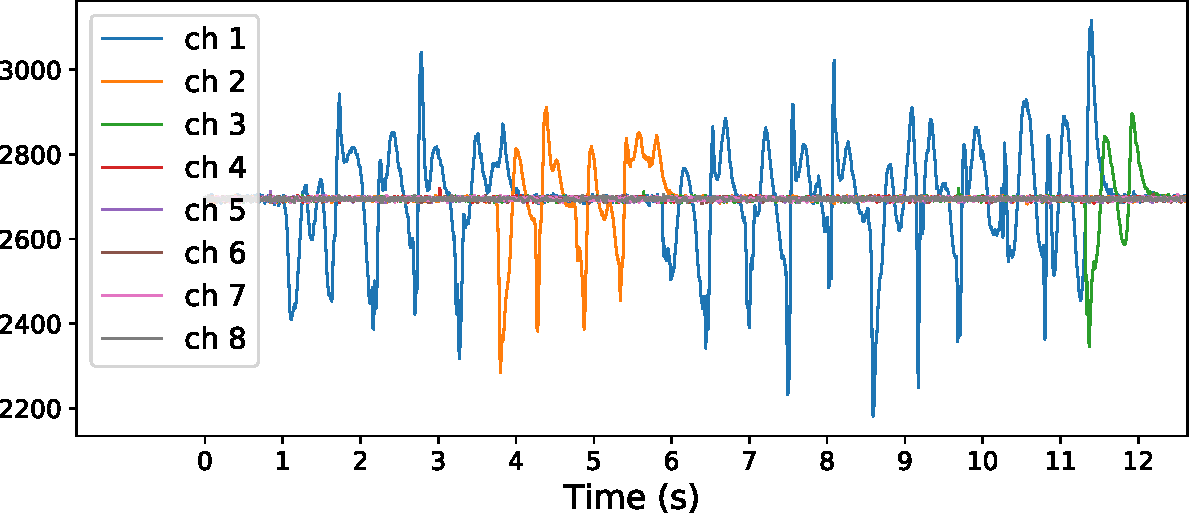
\includegraphics[trim= 0 0 0 0, width=0.8\linewidth, clip]{ex_signal_raw_2.pdf}
%             {\small Raw signal}
%         \medskip
%         \end{minipage}
%         \begin{minipage}{0.49\linewidth}
%         \centering
            \onslide<2->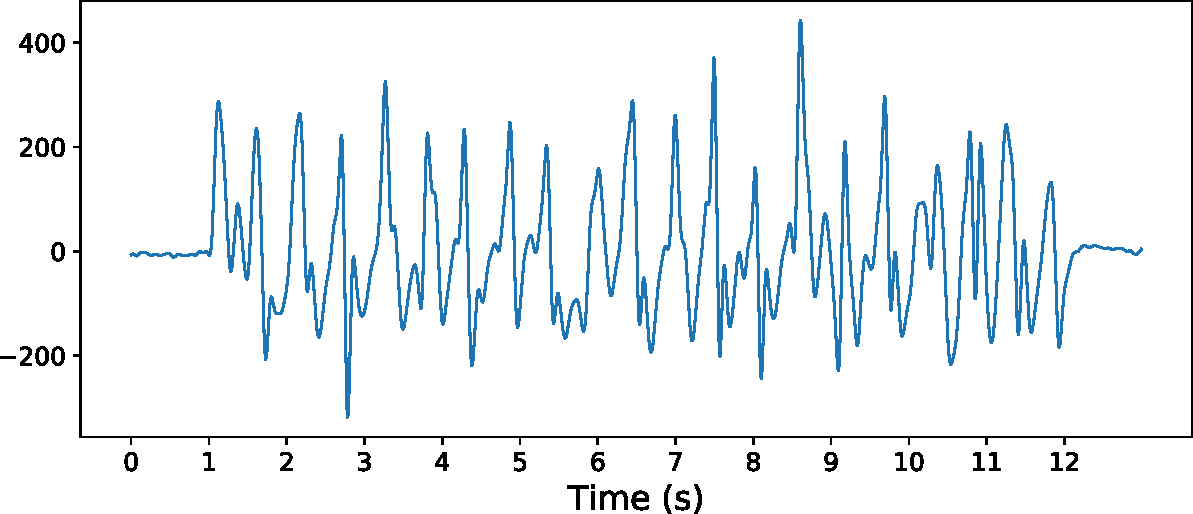
\includegraphics[trim= 0 0 0 0, width=0.8\linewidth, clip]{ex_signal_preproc_2.pdf}
%             {\small Preprocessed signal}
%         \medskip
%         \end{minipage}
    \end{overprint}
\end{minipage}\hfill
\begin{minipage}[t]{0.49\linewidth}
\vspace{0pt}
% \centering
%     \begin{itemize}
    \pause \pause
    \textbf{Experimental dataset}
    \begin{itemize}
        \item 28 volunteers aged 25 to 45
        \item 742 signals collected in \textbf{controlled environment}
        \item 55\% \emph{fall}, 45\% \emph{non-fall}
        \item varied fall events (forward, backward...) and activities of daily living (walking, sitting...)
    \end{itemize}
%     \end{itemize}
    \smallskip
    \centering
    \vspace{0.3cm}
    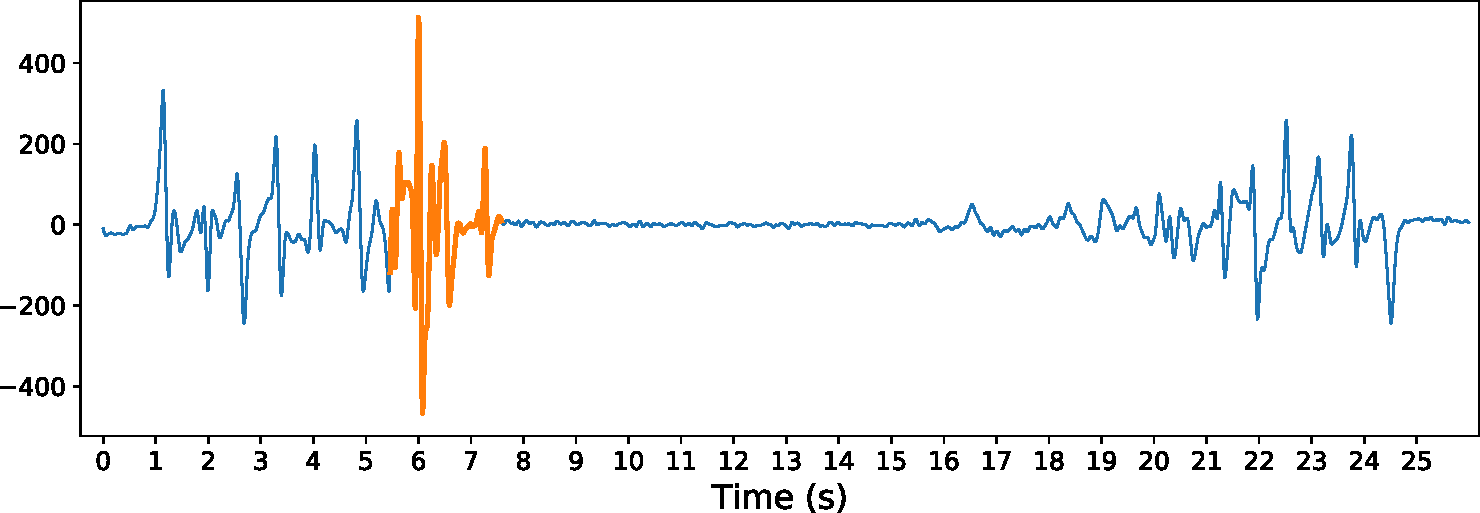
\includegraphics[width=0.9\textwidth]{ex_signal_chute_2.pdf}

\end{minipage}

\end{frame}

\subsection{Model}
\begin{frame}{Model}{}


\begin{minipage}[t]{0.49\linewidth}
    \vspace{0pt}
Time series as \emph{feature vector}. At every timestamp:
    \begin{enumerate}
        \item Window over the signal: 2.5 s
        \item Compute feature vector: 29 statistical measures (Min, Max, Shannon energy, Percentile,...) over three representations of the signal
    \end{enumerate}
    \centering
    \begin{overlayarea}{\linewidth}{0cm}
    \centering
    \only<1>{%
    \begin{tikzpicture}[line cap=round,line join=round,>=triangle 45,x=0.2cm,y=0.4cm]
    \node[inner sep=0pt] at (0,0)
        {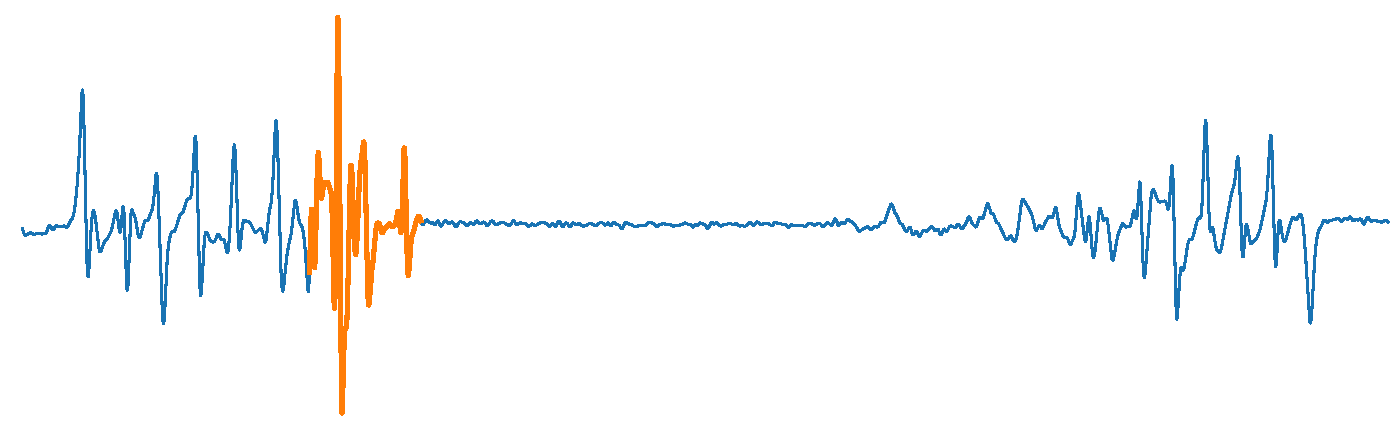
\includegraphics[width=0.55\linewidth, trim= 0 0 250 0, clip]{ex_signal_chute_2_epure.pdf}};
    \draw[color=gray!90,  line width=0.5pt] (-2.5,-2.1) rectangle (-0.5,2.2);
    \coordinate (A) at (-1.6,-2.5);
    \draw[->, >=stealth] (A) -- (-4.4,-4);
    \draw[->, >=stealth] (A) -- (-1.6,-4);
    \draw[->, >=stealth] (A) -- (1.2,-4);
    \draw (-5.5,-4.9) node[right]{$s$};
    \draw (-3.5,-4.9) node[right]{$\frac{d}{dt}s$};
    \draw (-0.5,-4.9) node[right]{$\mathcal{F}(s)$};
    \draw[->, >=stealth] (-1.6,-5.8) -- (-1.6,-6.5)
node[midway,below,yshift=-3pt]{\small Min, Max, Energy...};
    \path[draw,decorate,decoration=brace] (4.5,-7.5) -- (-7.5,-7.5)
node[midway,below,yshift=-3pt]{$\mathbf{x} \in \RR^{87}$};
    \end{tikzpicture}%
    }%
    \only<2->{%
    \begin{tikzpicture}[line cap=round,line join=round,>=triangle 45,x=0.2cm,y=0.4cm]
    \node[inner sep=0pt] at (0,0)
        {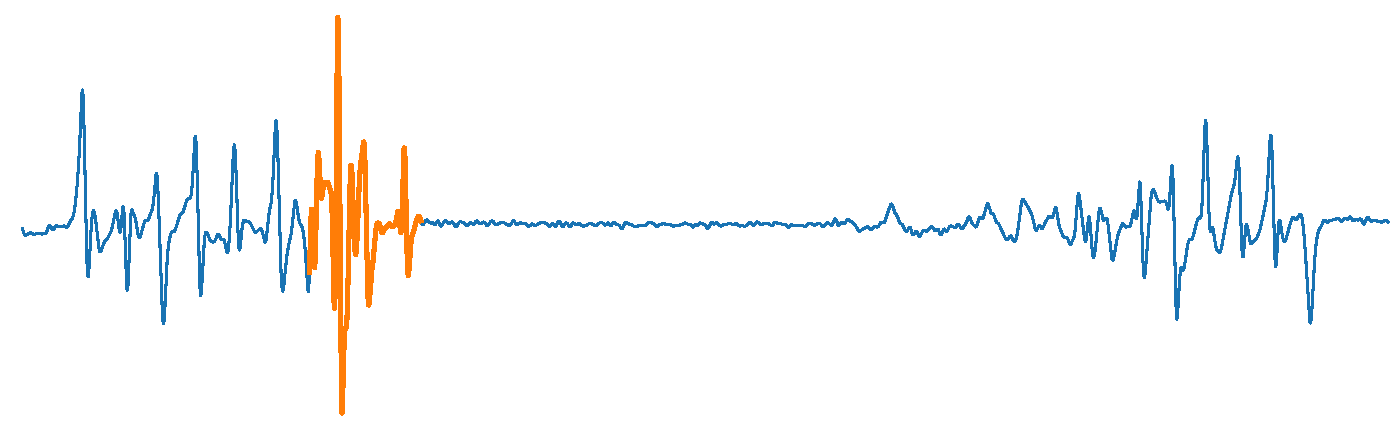
\includegraphics[width=0.55\linewidth, trim= 0 0 250 0, clip]{ex_signal_chute_2_epure.pdf}};
    \draw[color=gray!90,  line width=0.5pt] (-2.5,-2.1) rectangle (-0.5,2.2);
    \coordinate (A) at (-1.6,-2.5);
    \draw[->, >=stealth] (A) -- (-1.6,-3.5);
    \draw (-3.5,-4) node[right]{$x \in \RR^{87}$};
    \end{tikzpicture}
    }%
    \end{overlayarea}
    
    \vspace{3cm}
    \pause[2]
    \begin{enumerate}
        \item[3.] Classification model: Random Forest (\citet{Breiman2001}), based on \textbf{decision trees}
        
%     \textbf{Random Forest}: Aggregation of \textbf{decision trees}.
    \end{enumerate}
\end{minipage}\hfill
\begin{minipage}[t]{0.49\linewidth}
    \vspace{0pt}
    \begin{tcolorbox}[title=Decision tree,size=title,boxrule=0.2pt]
    \small
    Feature space $\XX = \RR^Q$.
    Division of $\XX$ into non-overlapping regions $R_1,...,R_J$.
    Algorithm CART: recursive binary splits \cite{breiman84} that solve:
    \begin{gather*}
        \argmax_{X_{q}, \tau} \IG\;,  \;\;\;\text{\small{(information gain)}}\\
        \text{with} \quad \IG(X_{q}, \tau) = I(n) - \frac{N_{l}}{N_n}I(l) - \frac{N_{r}}{N_{n}}I(r)\;,\\
        \text{and} \quad I(n) = \mathrm{Gini}(n) = \sum_{k}p_{nk}(1-p_{nk})\;.
    \end{gather*}
    \end{tcolorbox}
    \begin{minipage}[t]{0.49\linewidth}
        \vspace{-5pt}
        \centering
        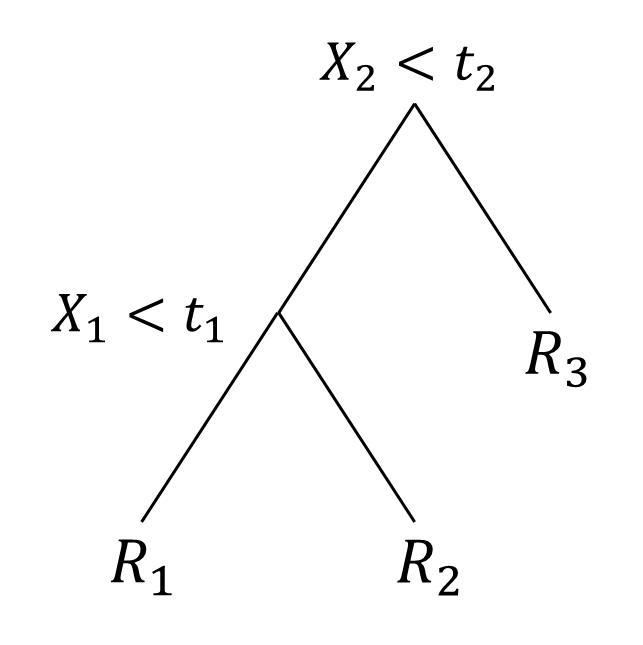
\includegraphics[width=0.65\linewidth, trim= 0 0 0 0, clip]{schema_decision_tree_1.png}\\
%     {\small Tree}
    \end{minipage}
    \begin{minipage}[t]{0.49\linewidth}
        \vspace{-5pt}
        \centering
        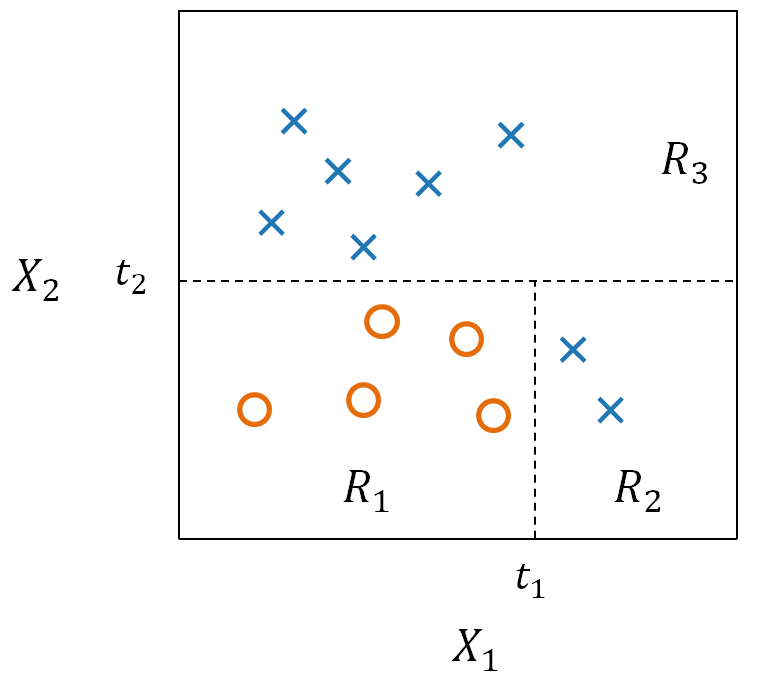
\includegraphics[width=0.9\linewidth, trim= 0 0 0 0, clip]{schema_decision_tree_3.png}\\
%     {\small Regions}
    \end{minipage}
    \centering
    \small
    Predicion function:\;
    $f(x) = \sum_{j=1}^{J}c_{j}\mathbbm{1}(x\in R_{j})$

\end{minipage}
\end{frame}

\begin{frame}{Model}{}
\begin{minipage}[t]{0.45\linewidth}
    \vspace{0pt}
    \begin{tcolorbox}[title=Random forest,size=title,boxrule=0.2pt]
        Decision trees $d_1,...,d_{N_T}$ grown with two rules:
        \begin{itemize}
            \item Each tree is trained with a \emph{bootstrap} of the training set
            \item At each split, access to a random subset of pool of features
        \end{itemize}
        Each tree is a ``vote'' for a class.
%         The prediction function is then
%         \begin{gather*}
%         f(x) = \argmax_{k}f_{k}(x)\;,\\
%         \text{with} \quad f_{k}(x) = \frac{1}{N_T}\sum_{i=1}^{N_T}\mathbbm{1}(d_i(x)=k)
%         \end{gather*}
        The estimated probability of belonging to class $k$ is then:
        \begin{equation*}
            f_{k}(x) = \frac{1}{N_T}\sum_{i=1}^{N_T}\mathbbm{1}(d_i(x)=k)
        \end{equation*}

    \end{tcolorbox}
\end{minipage}\hfill
\begin{minipage}[t]{0.52\linewidth}
    \vspace{0pt}
%     \medskip
    \pause
    \centering\textbf{Data augmentation}\\
    Select $r$ windows in training signals

    \centering
    \begin{tikzpicture}[line cap=round,line join=round,>=triangle 45,x=0.2cm,y=0.4cm]
    \node[inner sep=0pt] at (0,0)
        {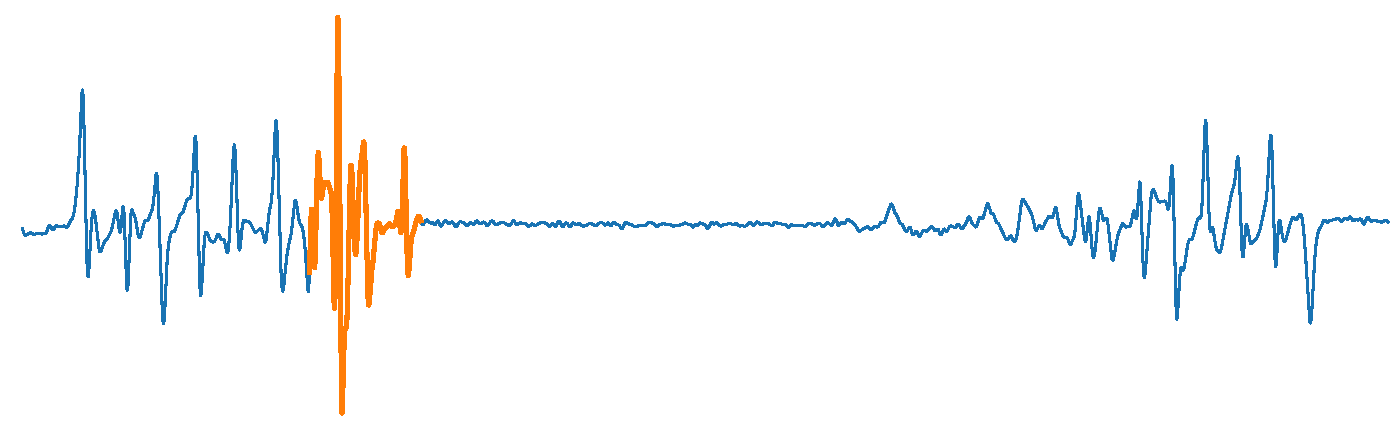
\includegraphics[width=0.55\linewidth, trim= 0 0 250 0, clip]{ex_signal_chute_2_epure.pdf}};
    \onslide<2>\draw[color=gray!90,  line width=0.5pt] (-3.3,-2.1) rectangle (-0.5,2.2);
    \onslide<3>\draw[color=gray!90,  line width=0.5pt] (-2.5,-2.1) rectangle (0.3,2.2);
    \onslide<4->\draw[color=gray!90,  line width=0.5pt] (-2.9,-2.1) rectangle (-0.1,2.2);
%     \draw (-2.5,-2.5) node[right]{$\mathbf{x} \in \RR^{87}$};
    \end{tikzpicture}
    
    \begin{overlayarea}{\linewidth}{1.25cm}
    \small
    \centering
    \only<2-4>{
    $\left[
    \begin{array}{ccc}
        x_{1,1} & ... & x_{1,Q} \\
        \onslide<3-4>{x_{2,1} & ... & x_{2,Q}} \\
        \onslide<4>{x_{3,1} & ... & x_{3,Q}} \\
    \end{array}
    \right]
    $
    }
    \only<5->{
    $\left[
    \begin{array}{ccc}
        x_{1,1} & ... & x_{1,Q} \\
        \vdots & & \vdots \\
        x_{r,1} & ... & x_{r,Q} \\
    \end{array}
    \right]
    $
    }
    \end{overlayarea}
    \begin{itemize}
        \item \textit{Fall} signals: encompass the fall
        \item \textit{Non-fall} signals: random location
    \end{itemize}


\end{minipage}



\end{frame}

\begin{frame}{Model}{Time aggregation}

\centering
\begin{minipage}[t]{0.7\linewidth}
    \centering
    \vspace{0pt}
    \renewcommand{\ratio}{0.5}
%     \begin{overlayarea}{\linewidth}{0cm} %{width}{height}
    \begin{overprint}
        
        \onslide<1-2>
        \centering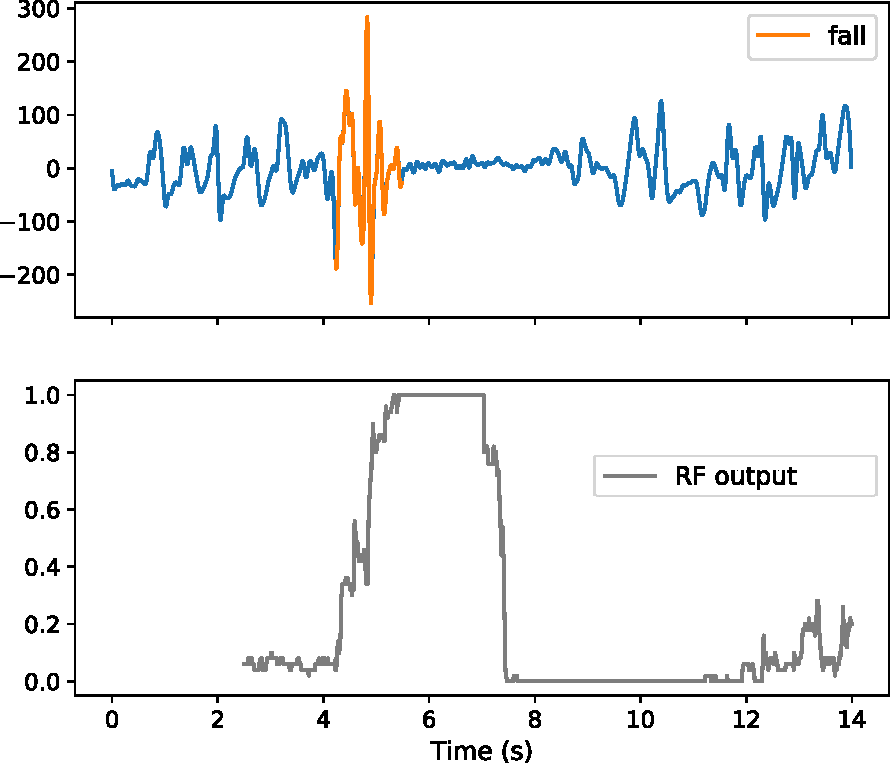
\includegraphics[width=\ratio\linewidth]{20140925a-1101-1115-FallLateral-Lateral-Yamina_begin_423_end_549_RFresponse_TP_beforebuff_noth.pdf}
        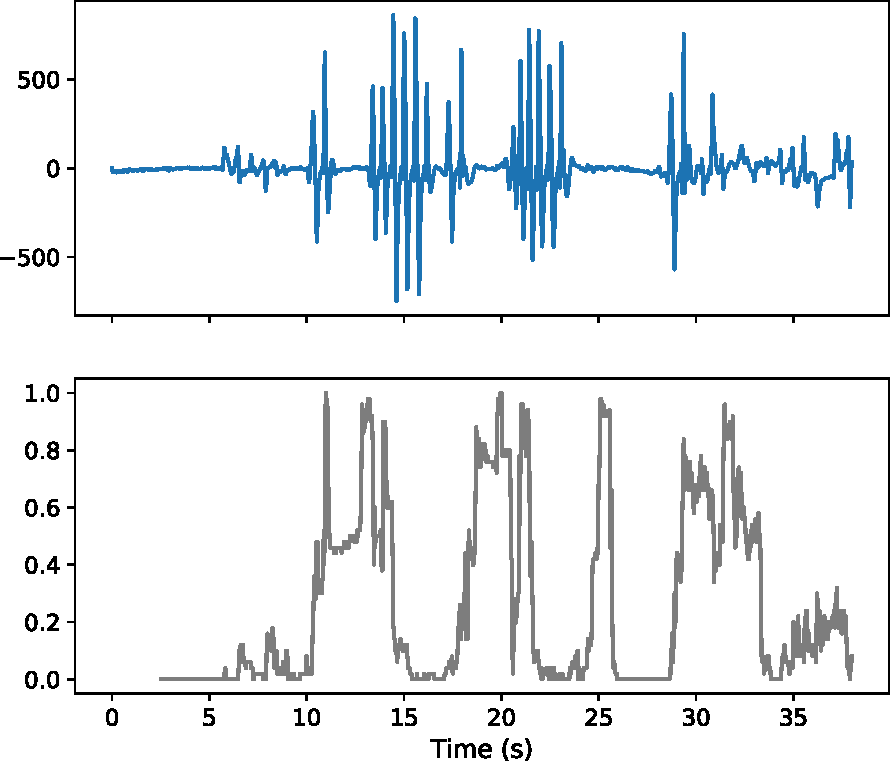
\includegraphics[width=\ratio\linewidth]{20140925a-0905-0943-Jump1-Yamina_RFresponse_TN_beforebuff_noleg_noth.pdf}
        \onslide<3->
        \centering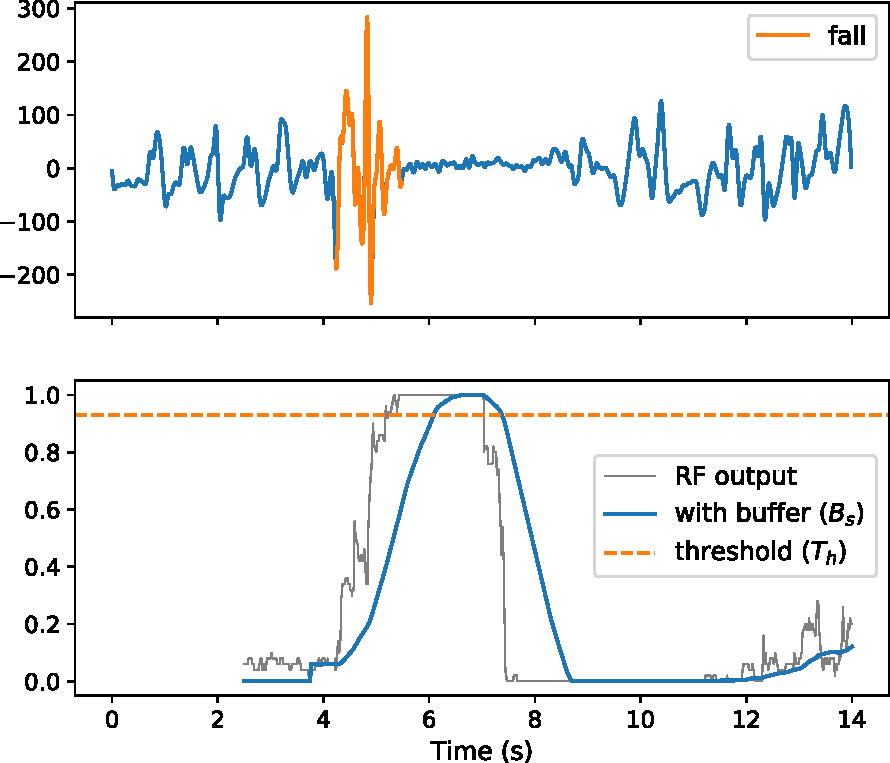
\includegraphics[width=\ratio\linewidth]{20140925a-1101-1115-FallLateral-Lateral-Yamina_begin_423_end_549_RFresponse_TP.pdf}
        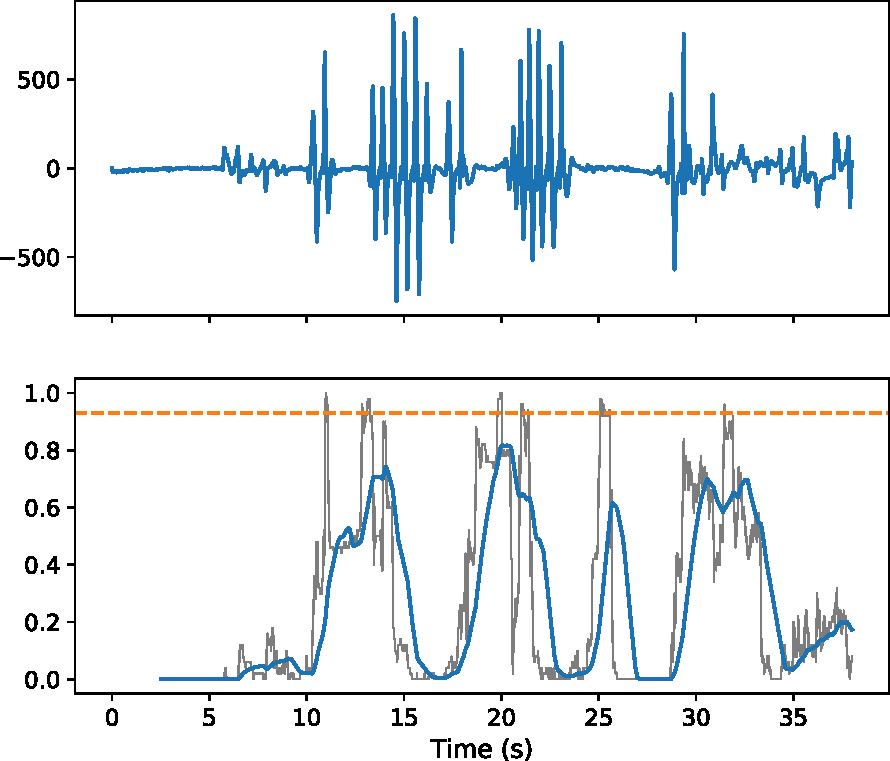
\includegraphics[width=\ratio\linewidth]{20140925a-0905-0943-Jump1-Yamina_RFresponse_TN.pdf}
%     \end{overlayarea}
    \end{overprint}

\end{minipage}

    \pause
    \medskip
    \centering\textbf{Time aggregation}
    
    \raggedright
    
    \centering
    \begin{minipage}[t]{0.42\linewidth}
        \vspace{0pt}
        $N_f(t)$ : number of trees voting for \emph{fall}\\
        Use a buffer $B_s \in \NN$ and a threshold $T_h \in [0, 1]$
        \begin{equation*}
        g(t) = \frac{\sum\limits_{u=t-B_{s}+1}^{t}N_{f}(u)}{B_{s}\times N_{T}}\\
        \end{equation*}
    \end{minipage}\hspace{0.2cm}
    \begin{minipage}[t]{0.42\linewidth}
        \vspace{0pt}
        New binary classification function:
        \begin{equation*}
        d(t) = 
        \begin{cases}
        1, & \textit{if}\ g(t) > T_{h} \\
        0, & \textit{otherwise}
        \end{cases}
        \end{equation*}
    \end{minipage}

\end{frame}

\begin{frame}{Model}{Parameters evaluation}
    
    \vspace{1.0cm}
    \renewcommand{\ratio}{0.32}
    \centering
    \begin{minipage}[t]{0.9\linewidth}
        \centering
        \begin{minipage}[t]{\ratio\linewidth}
            \centering
            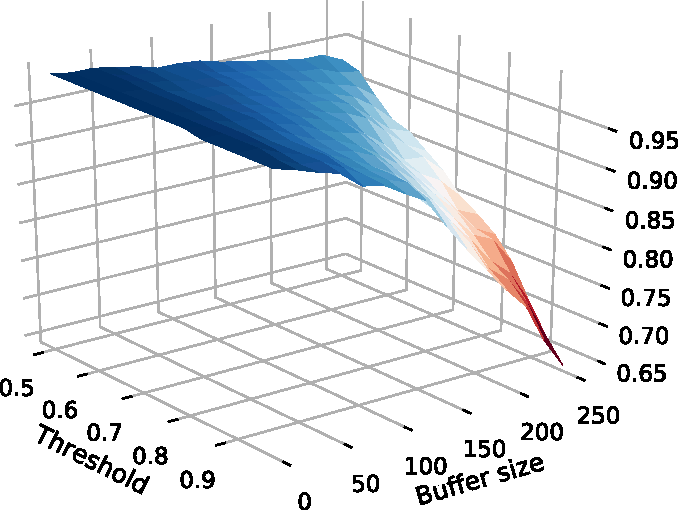
\includegraphics[width=\linewidth]{plot3d_compare_methods_buff_2019_12_05_14h51m35s_rf_TPR_view2.pdf}\\
            \smallskip
            {\small True positive rate}
        \end{minipage}
        \begin{minipage}[t]{\ratio\linewidth}
            \centering
            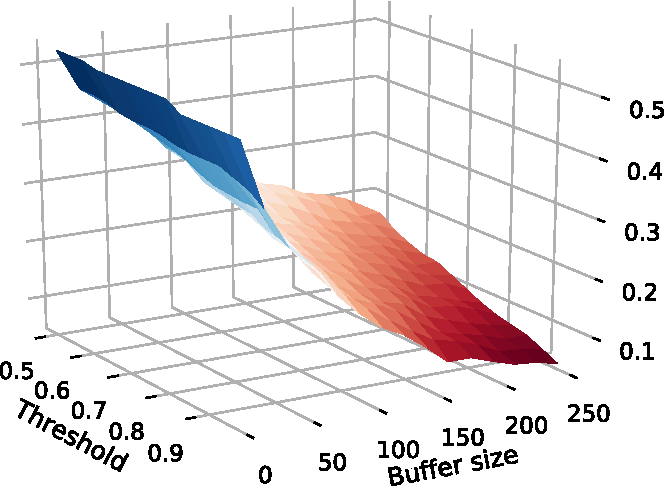
\includegraphics[width=\linewidth]{plot3d_compare_methods_buff_2019_12_05_14h51m35s_rf_FPR_view2.pdf}\\
            \smallskip
            {\small False positive rate}
        \end{minipage}
        \begin{minipage}[t]{\ratio\linewidth}
            \centering
            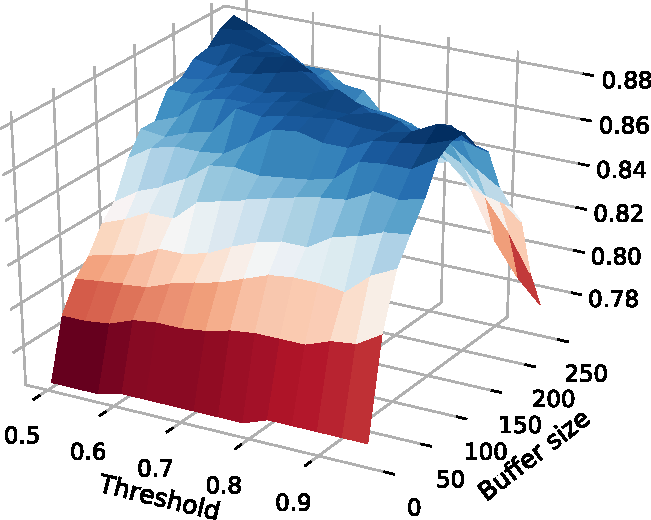
\includegraphics[width=0.92\linewidth]{plot3d_compare_methods_buff_2019_12_05_14h51m35s_rf_Accuracy.pdf}\\
            \smallskip
            {\small Accuracy}
        \end{minipage}
    \end{minipage}
    
    \medskip
    
    \begin{itemize}
    \centering
        \item Buffer/threshold trade-off useful for maintaining low FPR while improving TPR
    \end{itemize}

    \pause
    \vspace{0.5cm}
    Decision rule is ready. Is it implementable in the local processing unit ?

\end{frame}

\subsection{Feature selection}

\begin{frame}{Feature selection}

\begin{minipage}[t]{0.49\linewidth}
    \vspace{0pt}
    \begin{tcolorbox}[title=Feature importance,size=title,boxrule=0.2pt]
        \begin{gather*}
        \text{Tree: } I(X_{q}) = \sum_{\text{nodes}\ t}p(t)\Delta i(t)\mathbbm{1}(v(t)=X_{q})\\
        \text{Random forest: }I(X_{q}) = \frac{1}{N_{T}}\sum_{n=1}^{N_T}I(T_n, X_{q})
        \end{gather*}
    \end{tcolorbox}
    \only<3->{
    \begin{tcolorbox}[title=Recursive feature elimination,size=title,boxrule=0.2pt]
    Initial pool of $Q$ features $X_1, ..., X_Q$.
        \begin{enumerate}
            \item Train several times and record variable importances
            \item Average of importances over trainings. $X_{q}* = \argmin_{X_i} I(X_{i})$
            \item Remove $X_{q}*$ from the pool of features and back to step 1
        \end{enumerate}
    \end{tcolorbox}
    }
\end{minipage}\hfill
\begin{minipage}[t]{0.49\linewidth}
    \vspace{0pt}
    \begin{overlayarea}{\textwidth}{\textheight}
    \only<2-3>{
    \centerline{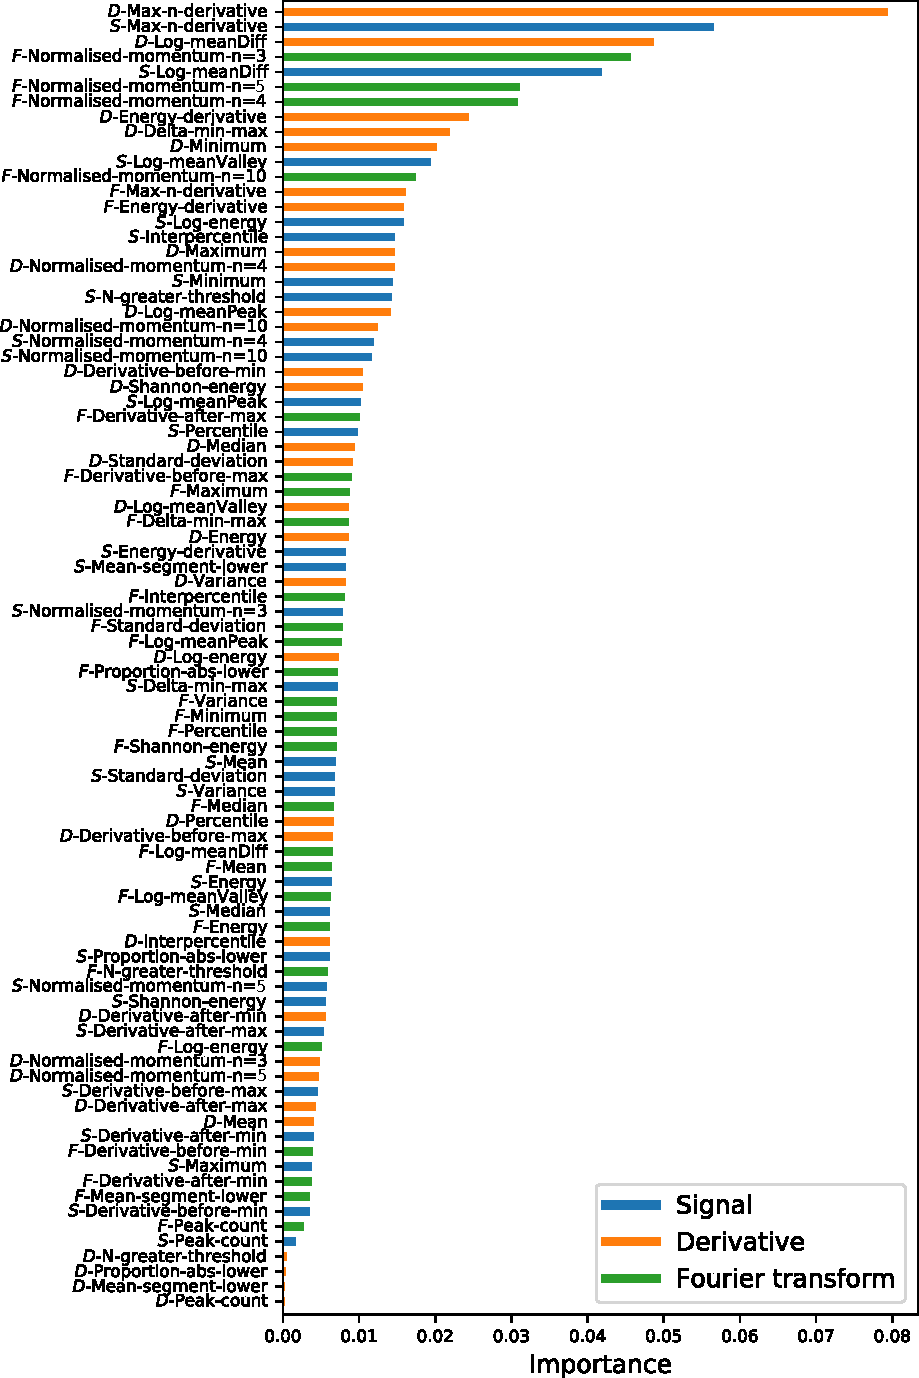
\includegraphics[width=0.75\linewidth, trim= 0 0 0 0, clip]{plot_feature_importance_all_epure.pdf}}
    }
    \only<4->{
    \vspace{1.0cm}
    \centerline{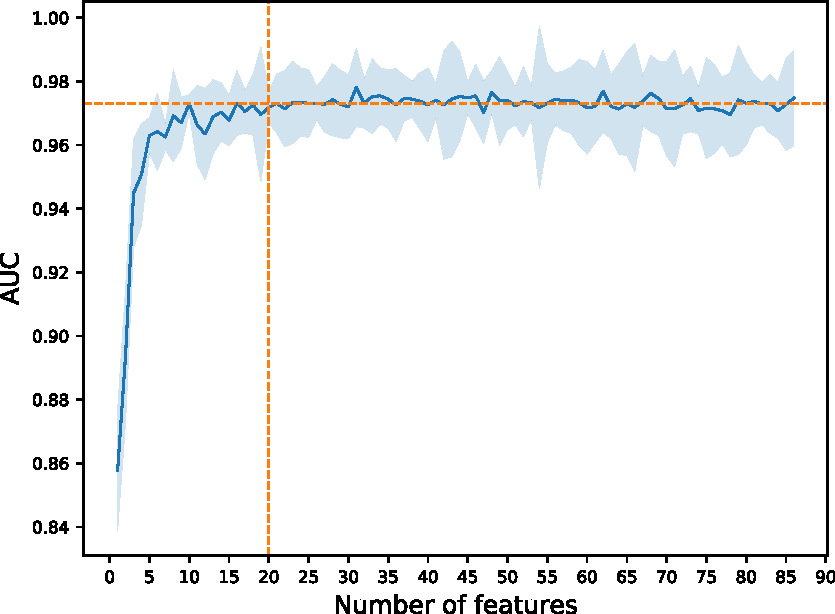
\includegraphics[width=0.9\linewidth]{plot_rf_feat_reduc_AUC_epure.pdf}}
    }
    \end{overlayarea}
\end{minipage}
\end{frame}

\subsection{Results}
\begin{frame}{Results}

\centering
\begin{minipage}[t]{0.7\linewidth}
\textbf{Set up}:
    \begin{itemize}
        \item Fixed params: $r$ set to 5 and $Q$ set to 20
        \item Varying $T_h$ (0.5 to 1) and $B_s$ (5 to 250)
        \item Record best Accuracy and show corresponding TPR, FPR
%         \onslide<1>{
%         \item If FPR is constrained to be max 10\%, what is the range of TPRs ?
%         }
    \end{itemize}
\end{minipage}

\smallskip

\begin{table}[ht]
\small
\begin{center}
\begin{tabular}{c c c c }
\toprule
  Model     & Accuracy & TPR & FPR \\
\midrule
LR   &  86.8 $\pm$ 1.5 & 90.5  $\pm$  2.4 &  17.7  $\pm$  4.9 \\
LDA   &  85.5  $\pm$  1.2  & 91.0  $\pm$  2.1 &  21.7  $\pm$  3.7 \\
k-NN  &    87.0  $\pm$  1.9 & 89.2  $\pm$  1.4  & \textbf{16.0  $\pm$  4.7} \\
SVM  &   87.6  $\pm$  3.2 & 90.0  $\pm$  4.5 & \textbf{15.5  $\pm$  6.8} \\
MLP  &\textbf{88.2  $\pm$  1.5} & \textbf{92.4  $\pm$  1.2} & 17.3  $\pm$  4.1 \\
RF  & \textbf{88.2  $\pm$  1.5} & \textbf{91.7 $\pm$ 3.5} & 16.2  $\pm$  6.2 \\
\bottomrule
\end{tabular}
% \begin{tabular}{c c c c | c c}
% \toprule
%   Model     & Accuracy & TPR & FPR & $\text{TPR}_{\text{min}}^{\text{FPR}<10}$ & $\text{TPR}_{\text{max}}^{\text{FPR}<10}$ \\
% \midrule
% LR   &  86.8 $\pm$ 1.5 & 90.5  $\pm$  2.4 &  17.7  $\pm$  4.9 & 67.0  $\pm$  10.8 & 80.4 $\pm$  6.4 \\
% LDA   &  85.5  $\pm$  1.2  & 91.0  $\pm$  2.1 &  21.7  $\pm$  3.7 & 56.9  $\pm$  7.0 & 78.7  $\pm$  3.8 \\
% k-NN  &    87.0  $\pm$  1.9 & 89.2  $\pm$  1.4  & \textbf{16.0  $\pm$  4.7} & 63.1  $\pm$  4.2 & 83.1  $\pm$  2.5 \\
% SVM  &   87.6  $\pm$  3.2 & 90.0  $\pm$  4.5 & \textbf{15.5  $\pm$  6.8} & 69.2 $\pm$ 2.1 & 82.9  $\pm$  3.2 \\
% MLP  &\textbf{88.2  $\pm$  1.5} & \textbf{92.4  $\pm$  1.2} & 17.3  $\pm$  4.1 & 71.4  $\pm$  4.5 & 85.1  $\pm$  2.1\\
% RF  & \textbf{88.2  $\pm$  1.5} & \textbf{91.7 $\pm$ 3.5} & 16.2  $\pm$  6.2 & 63.8  $\pm$  6.8 & 84.3  $\pm$  7.9 \\
% \bottomrule
% \end{tabular}
\end{center}
\end{table}

\begin{minipage}[t]{0.7\linewidth}
\textbf{Comments}:
    \begin{itemize}
        \item Parametric methods perform slightly worse than non-parametric
        %that contain variable selection (RF), feature space modification (SVM) or feature construction (MLP)
        \item RF is slightly better than others
%         \onslide<1>{
%         }
    \end{itemize}
\end{minipage}

\end{frame}